\documentclass[12pt]{book}

\title{Exercises for Think Java}
\author{J. David Eisenberg}

\newcommand{\thetitle}{Exercises for Think Java}
\newcommand{\thesubtitle}{How to Think Like a Computer Scientist}
\newcommand{\theauthors}{J. David Eisenberg}
\newcommand{\theversion}{1st Edition, Version 1.0.0}

%%%% Both LATEX and PLASTEX

\usepackage{graphicx}
\usepackage{setspace}
\usepackage[T1]{fontenc} 
\usepackage[utf8x]{inputenc}

% automatically index glossary terms
\newcommand{\term}[1]{%
\item[#1:]\index{#1}}

\usepackage{amsmath}
\usepackage{amsthm}

% format end of chapter excercises
\newtheoremstyle{exercise}
  {12pt}        % space above
  {12pt}        % space below
  {}            % body font
  {}            % indent amount
  {\bfseries}   % head font
  {}            % punctuation
  {12pt}        % head space
  {}            % custom head
\theoremstyle{exercise}
\newtheorem{exercise}{Exercise}[chapter]

\newif\ifplastex
\plastexfalse

%%%% PLASTEX ONLY
\ifplastex

\makeindex

\usepackage{localdef}

\usepackage{url}
\renewcommand{\href}[2]{\url{#1}}

\makeatletter
\newcount\anchorcnt
\newcommand*{\Anchor}[1]{%
  \@bsphack%
    \Hy@GlobalStepCount\anchorcnt%
    \edef\@currentHref{anchor.\the\anchorcnt}%
    \Hy@raisedlink{\hyper@anchorstart{\@currentHref}\hyper@anchorend}%
    \M@gettitle{}\label{#1}%
    \@esphack%
}
\makeatother

% code listing environments:
% we don't need these for plastex because they get replaced
% by preprocess.py
%\newenvironment{code}{\begin{verbatim}}{\end{verbatim}}
%\newenvironment{stdout}{\begin{verbatim}}{\end{verbatim}}

% inline syntax formatting
%\newcommand{\java}{\verb}%}
%\newcommand{\java}{\texttt}%}
\newcommand{\java}[1]{{\tt #1}}%{
\newcommand{\textcolor}[1]{\relax}

%%%% LATEX/HTML ONLY
\else

%BEGIN LATEX
\usepackage{comment}
\excludecomment{htmlonly}
\includecomment{latexonly}
%END LATEX

\usepackage{geometry}
\geometry{
    %paperwidth=6.0in,
    %paperheight=9.0in,
    width=5.5in,
    height=8.5in,
    hmarginratio=1:1,  % 3:2 for binding offset
    vmarginratio=1:1,
    includehead=true,
    headheight=15pt
}

% index with headings
\usepackage{imakeidx}
\makeindex[options= -s headings.ist]

% paragraph spacing
\setlength{\parindent}{0pt}                      % 17.62482pt
\setlength{\parskip}{12pt plus 4pt minus 4pt}    % 0.0pt plus 1.0pt
\linespread{1.05}
\def\arraystretch{1.5}

% list spacing
\setlength{\topsep}{5pt plus 2pt minus 3pt}      % 10.0pt plus 4.0pt minus 6.0pt
\setlength{\partopsep}{-6pt plus 2pt minus 2pt}  %  3.0pt plus 2.0pt minus 2.0pt
\setlength{\itemsep}{0pt}                        %  5.0pt plus 2.5pt minus 1.0pt

% these are copied from tex/latex/base/book.cls
% all I changed is afterskip
\makeatletter
\renewcommand{\section}{\@startsection{section}{1}{\z@}%
    {-3.5ex \@plus -1ex \@minus -.2ex}%
    {0.7ex \@plus.2ex}%
    {\normalfont\Large\bfseries}}
\renewcommand\subsection{\@startsection{subsection}{2}{\z@}%
    {-3.25ex\@plus -1ex \@minus -.2ex}%
    {0.3ex \@plus .2ex}%
    {\normalfont\large\bfseries}}
\renewcommand\subsubsection{\@startsection{subsubsection}{3}{\z@}%
    {-3.25ex\@plus -1ex \@minus -.2ex}%
    {0.3ex \@plus .2ex}%
    {\normalfont\normalsize\bfseries}}
\makeatother

% table of contents vertical spacing
\usepackage{tocloft}
\setlength\cftparskip{8pt plus 4pt minus 4pt}

% balanced index with TOC entry
\usepackage[totoc]{idxlayout}

% The following line adds a little extra space to the column
% in which the Section numbers appear in the table of contents
\makeatletter
\renewcommand{\l@section}{\@dottedtocline{1}{1.5em}{3.0em}}
\makeatother

% customize page headers
\usepackage{fancyhdr}
\pagestyle{fancyplain}
\renewcommand{\chaptermark}[1]{\markboth{Chapter \thechapter ~~ #1}{}}
\renewcommand{\sectionmark}[1]{\markright{\thesection ~~ #1}}
\lhead[\fancyplain{}{\bfseries\thepage}]%
      {\fancyplain{}{\bfseries\rightmark}}
\rhead[\fancyplain{}{\bfseries\leftmark}]%
      {\fancyplain{}{\bfseries\thepage}}
\cfoot{}
%\usepackage[mmddyyyy]{datetime}
%\rfoot{\textcolor{gray}{\tiny \thetitle, \theversion, \today}}

%% tweak spacing of figures and captions
%\usepackage{floatrow}
%\usepackage{caption}
%\captionsetup{
%    font=small,
%    labelformat=empty,
%    justification=centering,
%    skip=4pt
%}

% colors for code listings and output
\usepackage{xcolor}
\definecolor{bgcolor}{HTML}{FAFAFA}
\definecolor{comment}{HTML}{007C00}
\definecolor{keyword}{HTML}{0000FF}
\definecolor{strings}{HTML}{B20000}

% syntax highlighting in code listings
\usepackage{textcomp}
\usepackage{listings}
\lstset{
    language=java,
    basicstyle=\ttfamily,
    backgroundcolor=\color{bgcolor},
    commentstyle=\color{comment},
    keywordstyle=\color{keyword},
    stringstyle=\color{strings},
    columns=fullflexible,
    emph={label},  % keyword?
    keepspaces=true,
    showstringspaces=false,
    upquote=true,
    xleftmargin=15pt,  % \parindent
    framexleftmargin=3pt,
    aboveskip=\parskip,
    belowskip=\parskip
}

%\usepackage{newunicodechar}
%\newunicodechar{′}{${^\prime}$}
\DeclareUnicodeCharacter{2032}{$^\prime$}
\DeclareUnicodeCharacter{2033}{$^{\prime\prime}$}
% code listing environments
\lstnewenvironment{code}
{\minipage{\linewidth}}
{\endminipage}
\lstnewenvironment{stdout}
{\lstset{commentstyle=,keywordstyle=,stringstyle=,extendedchars=true,
literate={°}{$^{\circ}$}1
 {′}{$^{\prime}$}1
 {″}{$^{\prime\prime}$}2
 }
\minipage{\linewidth}}
{\endminipage}
% literate={°}{$^{\circ}$}
% interactive code listing
\lstnewenvironment{trinket}[2][400]
{\minipage{\linewidth}}
{\endminipage}

% inline syntax formatting
\newcommand{\java}[1]{\lstinline{#1}}%{

% prevent hyphens in names
\hyphenation{DrJava}
\hyphenation{GitHub}
\hyphenation{Javadoc}

% pdf hyperlinks, table of contents, and document properties
\usepackage{hyperref}
\hypersetup{%
  pdftitle={\thetitle: \thesubtitle},
  pdfauthor={\theauthors},
  pdfsubject={\theversion},
  pdfkeywords={},
  bookmarksopen=false,
  bookmarksnumbered=true,
  colorlinks=true,
  citecolor=black,
  filecolor=black,
  linkcolor=black,
  urlcolor=blue
}

% add dot after numbers in pdf bookmarks
\makeatletter
\renewcommand{\Hy@numberline}[1]{#1. }
\makeatother

\raggedbottom


\fi

%%%% END OF PREAMBLE
\begin{document}

\frontmatter

%%%% PLASTEX ONLY
\ifplastex

\maketitle

%%%% LATEX/HTML ONLY
\else

\begin{latexonly}

%--half title-------------------------------------------------
\thispagestyle{empty}

\begin{flushright}
\vspace*{2.0in}

\begin{spacing}{3}
{\huge \thetitle} \\
{\Large \thesubtitle}
\end{spacing}

\vspace{0.25in}

\theversion

\vfill
\end{flushright}

%--verso------------------------------------------------------
\newpage
\thispagestyle{empty}

\quad

%--title page-------------------------------------------------
\newpage
\thispagestyle{empty}

\begin{flushright}
\vspace*{2.0in}

\begin{spacing}{3}
{\huge \thetitle} \\
{\Large \thesubtitle}
\end{spacing}

\vspace{0.25in}

\theversion

\vspace{1in}

{\Large \theauthors}

% \vspace{0.5in}

% {\Large Green Tea Press}

% {\small Needham, Massachusetts}

\vfill
\end{flushright}

%--copyright--------------------------------------------------
\newpage
\thispagestyle{empty}

Copyright \copyright ~2021--2022 \theauthors.

\vspace{0.2in}

% \begin{flushleft}
% Green Tea Press \\
% 9 Washburn Ave \\
% Needham, MA 02492
% \end{flushleft}

Permission is granted to copy, distribute, and/or modify this work under the terms of the Creative Commons Attribution-NonCommercial-ShareAlike 4.0 International License, which is available at \url{https://creativecommons.org/licenses/by-nc-sa/4.0/}.

The original form of this book is \LaTeX\ source code.
Compiling this code has the effect of generating a device-independent representation of the book, which can be converted to other formats and printed.

The \LaTeX\ source for this book is available from \url{https://github.com/jdeisenberg/ThinkJava2Exercises}.

%--table of contents------------------------------------------

\cleardoublepage
\setcounter{tocdepth}{1}
\tableofcontents

\end{latexonly}

%--HTML title page--------------------------------------------

\begin{htmlonly}

\vspace{1em}

{\Large \thetitle: \thesubtitle}

{\large \theauthors}

\theversion

\vspace{1em}

Copyright \copyright ~2021--2022 \theauthors.

Permission is granted to copy, distribute, and/or modify this work under the terms of the Creative Commons Attribution-NonCommercial-ShareAlike 4.0 International License, which is available at \url{https://creativecommons.org/licenses/by-nc-sa/4.0/}.

\vspace{1em}

\end{htmlonly}

%-------------------------------------------------------------

%%%% END OF THE PART WE SKIP FOR PLASTEX
\fi

\chapter*{Preface}

\markboth{PREFACE}{PREFACE}
\addcontentsline{toc}{chapter}{Preface}

{\it Exercises for Think Java} is a companion volume to {\it Think Java 2nd Edition} by Allen B. Downey and Chris Mayfield 
\url{https://greenteapress.com/wp/think-java-2e/}

Evergreen Valley College, where I teach, has been encouraging faculty to use low-cost or open source textbooks. In this spirit, the Computer Science department decided to use {\it Think Java} for our introductory Computer Science course. While the book met most of our needs, we wanted more exercises for students to practice programming. There were also some topics that we cover in our course that were not in the book. Thus, we decided to add some material and more exercises.

Instead of editing the original book, which is open source, I have decided to make this a separate book for two reasons:

\begin{enumerate}
\item Inserting many exercises, some of which require a great deal of explanation, breaks up the flow of the material. 
\item The modified book would no longer match the print version, which some students prefer to use.
\end{enumerate}

\section*{Using the Code Examples}
\label{code}

Most of the code examples in this book are available from a Git repository at \url{https://github.com/jdeisenberg/ThinkJava2ExCode}.
Git is a ``version control system'' that allows you to keep track of the files that make up a project.
A collection of files under Git's control is called a ``repository''.

\index{repository}
\index{GitHub}

GitHub is a hosting service that provides storage for Git repositories and a convenient web interface.
It provides several ways to work with the code:

\begin{itemize}

\item You can create a copy of the repository on GitHub by clicking the {\sf Fork} button.
If you don't already have a GitHub account, you'll need to create one.
After forking, you'll have your own repository on GitHub that you can use to keep track of code you write.
Then you can ``clone'' the repository, which downloads a copy of the files to your computer.

\item Alternatively, you could clone the original repository without forking.
If you choose this option, you don't need a GitHub account, but you won't be able to save your changes on GitHub.

\item If you don't want to use Git at all, you can download the code in a ZIP archive using the {\sf Clone} button on the GitHub page.

\end{itemize}

After you clone the repository or unzip the ZIP file, you should have a directory named {\it ThinkJava2ExCode} with a subdirectory for each chapter in the book that contains sample code.

%\medskip

If you have additional comments or ideas about the text, please send them to: \href{mailto:david.eisenberg@evc.edu}{\tt david.eisenberg@evc.edu}.

\hfill J David Eisenberg

\hfill July 2021


\mainmatter

%~ \part{Programming Fundamentals}

\chapter{Computer Programming}

\section{Exercises}

\begin{exercise}
This exercise will let you practice displaying information.  Write a program named \java{AboutMe.java} with a \java{main} method that prints following:

\begin{enumerate}
\item Your name.
\item Your favorite color.
\item Your favorite word, in double quotes.
\item Your favorite poem, at least three lines long (If your favorite poem is longer than ten lines, give only the first three to ten lines.)
\item The author of the poem. The name should be indented four spaces and preceded by a hyphen and a space. If you don't know who wrote the poem, use ``Anonymous'' as the author.
\end{enumerate}

Use complete sentences and blank lines for readability.  To print a blank line, use:

\java{System.out.println();}

The parentheses are required, even though there is nothing between them. If you don't believe me, leave them out and see what the compiler has to say about it!

Here is what the output of my solution looks like:

\begin{stdout}
My name is David Eisenberg.
My favorite color is purple.
My favorite word is "kinkajou".

My favorite poem:

Beneath these high Cathedral stairs
Lie the remains of Susan Pares.
Her name was Wiggs, it was not Pares,
But Pares was put to rhyme with stairs.
    - Edward Lear
\end{stdout}
\end{exercise}


\chapter{Variables and Operators}
\label{variables}

\begin{exercise}
\label{ex:age}
Use Java to find your approximate age in days.

\begin{enumerate}

\item Create a new program name {\it AgeInDays.java}.
Copy or type in something like the Hello World program and make sure you can compile and run it.

\item Write a program that creates variables named \java{years} and \java{days} which represent your age in years and your age in days. Both of these are integers.

\item Set the \java{years} to your current age in years.

\item Calculate the \java{days} as \java{years} times 365.

\item Print the age in years and days, properly labeled. Here is what the output might look like:

\begin{stdout}
I am 25 years old.
That is about 9125 days.
\end{stdout}
\end{enumerate}

\end{exercise}


\begin{exercise}
\label{ex:dewpoint}
The point of this exercise is to use Java's arithmetic operators to calculate the {\it dew point}---the temperature at which water begins to condense out of the air. The dew point formula is more complicated than the one in the preceding exercise.

\begin{enumerate}

\item Write a program that creates variables named \java{temperature} and \java{relHumidity} which represent the temperature in degrees Celsius and the relative humidity as a percentage from 0 to 100. These will be \java{double} values. Assign values to those variables that represent a temperature of 17$^\circ$C and a relative humidity of 30\%.

\item Display the value of each variable on a line by itself.
This is an intermediate step that is useful for checking that everything is working so far.
Compile and run your program before moving on.

\item Calculate the dew point temperature using this approximate formula:

\begin{equation*}
dewPoint = temperature - {{100 - relHumidity} \over 5}
\end{equation*}

and display the value of the result. The \java{dewPoint} variable will also be a \java{double}.

\item Display the result of the calculation, properly labeled. Here is what the output might look like. Your output does not have to match
this exactly, but it must reflect the same information.

\begin{stdout}
For air temperature of 17.0 degrees Celsius
and relative humidity of 25.0%
The dew point is 2.0 degrees Celsius.
\end{stdout}
\end{enumerate}

\end{exercise}

\begin{exercise}
\label{ex:heatindex}
This exercise uses a fairly large formula to calculate the {\it heat index}, a measurement of how hot it feels when the relative humidity is factored in with the temperature. The purpose of this exercise is to get you comfortable with doing complex calculations in Java.

\begin{enumerate}
\item Create a new program named {\it HeatIndex.java}.

\item Create variables named \java{t} and \java{rh}, where \java{t} stands for the temperature and \java{rh} stands for the relative humidity. Set the temperature to 30 degrees Celsius and the relative humidity to 75\%.

\item Ordinarily we would use longer variable names like \java{temperature} and \java{relHumidity} as in Exercise~\ref{ex:dewpoint}, but the length of the formula makes it easier to type when using short names. Write a comment in your Java program that says that you are using \java{t} to stand for the temperature in degrees Celsius and \java{rh} for relative humidity.

\item Calculate the heat index using this formula:
\begin{equation*}
\begin{array}{l}
heatIndex = -8.78469475556 + 1.61139411\cdot t + 2.338548839\cdot rh - \\
 \qquad {0.14611605}\cdot t \cdot rh - {0.012308094}\cdot t\cdot t - \\
 \qquad {0.0164248278}\cdot rh\cdot rh + 0.002211732\cdot t\cdot t\cdot rh + \\
 \qquad 0.00072546\cdot t\cdot rh\cdot rh {-} {0.000003582} \cdot t\cdot t\cdot rh\cdot rh
\end{array}
\end{equation*}

Don't put this entire equation on one line in Java. Instead, split it into several lines as shown here, or use temporary variables to hold the parts of the formula.

\item Display the result of the calculation. Here is what the output might look like.

\begin{stdout}
For air temperature of 30.0 degrees Celsius
and relative humidity of 75.0%
The heat index is 36.299647994439965 degrees Celsius.
\end{stdout}

\end{enumerate}
\end{exercise}


\chapter{Input and Output}

\begin{exercise}
Modify the program you wrote in Exercise~\ref{ex:age} to prompt the user for their age in years.
\end{exercise}

\begin{exercise}
Modify the program you wrote in Exercise~\ref{ex:dewpoint} to prompt the user for the air temperature and relative humidity. Use \java{printf} to display the dew point with one digit to the right of the decimal point.
\end{exercise}

\begin{exercise}
Modify the program you wrote in Exercise~\ref{ex:heatindex} to prompt the user for the air temperature and relative humidity. Use \java{printf} to display the heat index temperature with one digit to the right of the decimal point.
\end{exercise}

\begin{exercise}
\label{ex:electricvehicle1}
In the United States, the ``fuel efficiency'' of an electric vehicle is measured in miles per kilowatt-hour (kWh). In Canada and Europe, it is measured in kWh per 100km. Write a program that prompts the user for efficiency in miles/kWh . The program will then calculate and display the equivalent efficiency in terms of kwH per/100km. One kilometer equals 0.621371 mile (or, if you prefer, one mile equals 1.609341 km). Here is what the output might look like:

\begin{stdout}
Enter miles per kilowatt-hour: 4.5
That is equivalent to 13.81 kWh/100km.
\end{stdout}

\end{exercise}

\begin{exercise}
\label{ex:electricvehicle2}
In Canada and Europe, the ``fuel efficiency'' of an electric vehicle is measured in kWh per 100km. In the United States, it is measured in miles per kilowatt-hour (kWh).  Write a program that prompts the user for electric vehicle efficiency in kwH/100km and calculates the equivalent in terms of miles/kWh.  One kilometer equals 0.621371 mile (or, if you prefer, one mile equals 1.609341 km). Here is what the output might look like.

\begin{stdout}
Enter kilowatt-hours per 100km: 13.5
That is equivalent to 4.62 miles/kWh.
\end{stdout}
\end{exercise}


\begin{exercise} 
\label{ex:purchase}

The goal of this exercise is to calculate the price of an order given an item's price, the quantity purchased, and the sales tax.
When it's finished, it should work like this:

\begin{stdout}
Please enter the unit price of the item $2.45
Enter the number you wish to purchase: 5

Subtotal:     $12.25
Tax at 7.50%:   0.92
Total:        $13.17
\end{stdout}

Note: the dollar sign in the first line is part of the prompt; the user does not enter the dollar sign.
Use \java{printf} to display exactly two digits to the right of the decimal point.

\end{exercise}


\begin{exercise}
\label{ex.degrees}
Because the \java{Scanner} class views input as a stream of characters, you can ask users for multiple inputs with a single prompt. For example, instead of asking the user for the width and height of a rectangle as two inputs in this code fragment:

\begin{code}
// ask for length in cm
System.out.print("Enter width of rectangle in cm: ");
double width = input.nextDouble();
        
System.out.print("Enter height of rectangle in cm: ");
double height = input.nextDouble();
\end{code}

Which looks like this when the program runs:

\begin{stdout}
Enter width of rectangle in cm: 5.3
Enter height of rectangle in cm: 2.6
\end{stdout}

You could use one prompt:

\begin{code}
System.out.println("Enter width and height of rectangle");
System.out.print("in cm separated by spaces: ");
double width = input.nextDouble();
double height = input.nextDouble();
\end{code}

Which looks like this when the program runs:

\begin{stdout}
Enter width and height of rectangle
in cm separated by spaces: 5.3 2.6
\end{stdout}

In this exercise, you will prompt the user to enter an angle as degrees, minutes, and seconds and convert it to decimal degrees. Here is what the output might look like:

\begin{stdout}
Enter degrees, minutes, and seconds
separated by spaces: 25 15 30
That is 25.2583 degrees (decimal).
\end{stdout}

You may use either one prompt, as shown here, or three separate prompts.

\end{exercise}

\begin{exercise}
\label{brakingDistance}

This is another exercise that uses input and arithmetic operators to calculate the stopping distance for a vehicle. Write a program that prompts the user to enter:

\begin{itemize}

\item The initial velocity in kilometers per hour (\java{double}). A velocity of 60 miles per hour works out to about 97 kilometers per hour.
\item The reaction time in seconds (\java{double}). For most people, the reaction time is about 1.5 seconds.
\item The coefficient of friction for the tires (\java{double}). This is a dimensionless number, normally about 0.7.

\end{itemize}

Calculate and display the stopping distance using this formula:
$d = v \cdot t + {v^2 \over {2 \mu g}}$
where $t$ is the reaction time, $v$ is the initial velocity in {\bf meters per second}, $\mu$ is the coefficient of friction between the tires and the roadway, and $g$ is the acceleration of gravity in meters per second squared. Make $g$ a constant with the value 9.80665.

Notice that, since you are asking for the velocity in kilometers per hour, you must convert it to meters per second. Define constants \java{METERS_PER_KM} (1000) and \java{SECONDS_PER_HOUR} (3600) to use in this calculation.

Here is an example of what the program should look like:

\begin{stdout}
Stopping Distance Calculator
Enter velocity of vehicle in kilometers per hour: 97
Enter reaction time in seconds (normal is 1.5): 1.1
Enter coefficient of friction (from 0.1 to 1.0; normal 0.7): 0.5

Stopping distance is 103 meters.
\end{stdout}

In this program, it is better to use three separate prompts for the input because, unlike Exercise~\ref{ex.degrees}, the entries are not closely related to each other.
 
\end{exercise}

\begin{exercise}
The goal of this exercise is to show the need for planning a program. The calculations themselves are not sophisticated, but figuring out {\em what} those calculations are requires some thinking.

Consider a staircase as shown in Figure~\ref{fig.staircase}.

\begin{figure}[!h]
\begin{center}
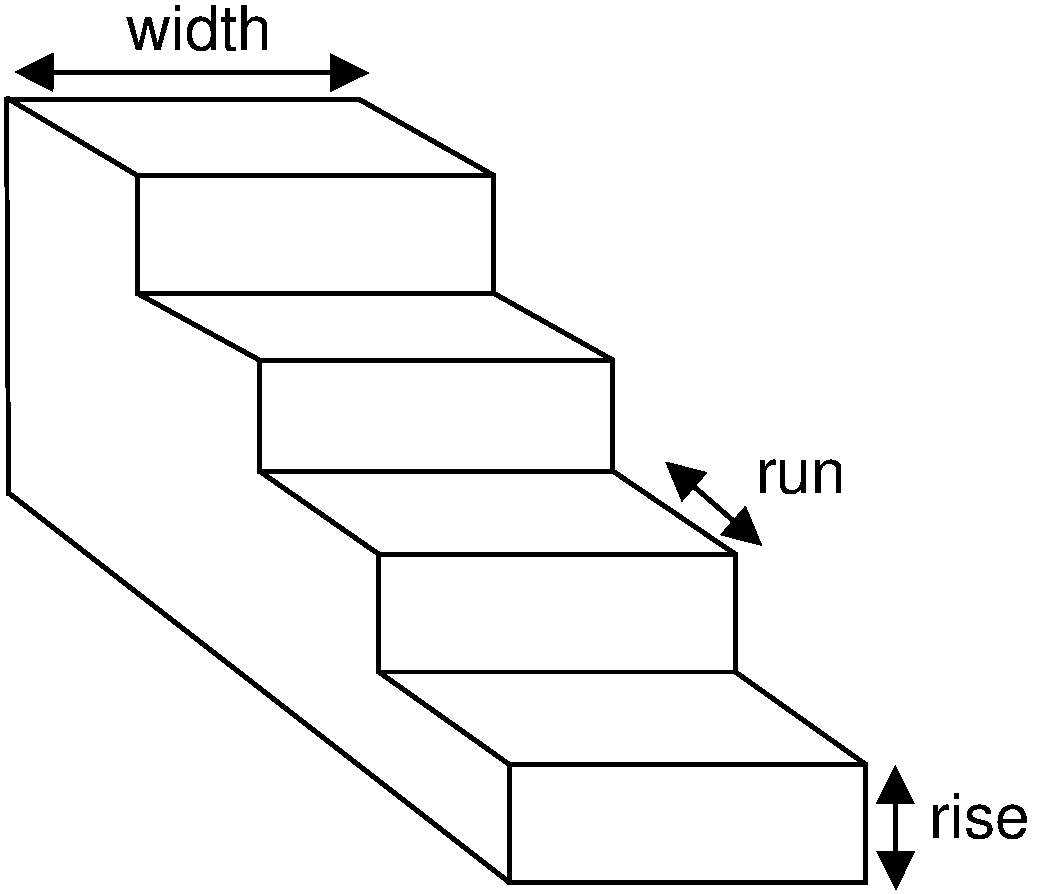
\includegraphics[scale=0.3]{figs/staircase.pdf}
\caption{A staircase showing the width, the {\em rise} (height), and the {\em run} (depth) of a step.}
\label{fig.staircase}
\end{center}
\end{figure}

Your job is to write a program that prompts the user for the number of steps in the staircase. It will then prompt for and read the width, rise, and run of a step in centimeters. The program will then calculate the number of cubic centimeters of concrete necessary to build the staircase. Round the number of cubic centimeters by adding 0.5 to the calculated volume and then casting that result to an integer.  In general,

\begin{code}
double x;
int xRounded = (int) (x + 0.5);
\end{code}

Calculate by hand what the result of this code would be when \java{x} is 3.4 and again when \java{x} is 3.6 to understand why this code works.

{\em Hints:} How many ``blocks'' the size of the bottom step do you need to build the staircase? Drawing a diagram {\em really} helps. To find the sum of the numbers 1 through n, use this formula: $sum = {{n(n+1)}\over 2}$

Here is what program output might look like:

\begin{stdout}
Staircase Volume Calculator
How many steps in the staircase? 5
Enter step width in cm: 45
Enter run of the step in cm: 20
Enter rise of the step in cm: 7.5
Total volume is 101250 cubic centimeters.
\end{stdout}
\end{exercise}




\chapter{Methods and Testing}

\begin{exercise}
Presume you are selling a product that has a particular cost to build (say, \$7.50) and a price that you charge the customer (say, \$10.00). There are two ways to calculate your profit: profit off the bottom, which uses this formula:

\begin{equation*}
bottom = 100 \cdot {(sellingPrice - costToBuild) \over costToBuild}
\end{equation*}

You can also have profit off the top, which uses this formula:

\begin{equation*}
top = 100 \cdot {(sellingPrice - costToBuild) \over sellingPrice}
\end{equation*}

In our example, the profit off the bottom is 33$1\over 3$\% and the profit off the top is 25\%.

Write methods named \java{profitOffTop} and \java{profitOffBottom}, both of which take the cost to build and selling price as \java{double} parameters and return the percentage as a \java{double}.

Your \java{main} method will ask the user for the cost to build and selling price. It will then calculate both profits and display them, properly labeled, with one digit to the right of the decimal point.
Here is what the output might look like:

\begin{stdout}
Enter cost to build: $7.50
Enter selling price: $10
The profit off the bottom is 33.3%.
The profit off the top is 25.0%
\end{stdout}

{\it Hint}: to output a percent sign using \java{printf}, use two percent signs in a row. For example:

\begin{code}
double result = 0.12 * 37.0;
System.out.printf("12%% of 37 is %.1f\n", result);
\end{code}

\end{exercise}

\begin{exercise}
To determine the focal length of a camera lens, you use this formula:

\begin{equation*}
{1 \over f} = {1 \over d_o} + {1 \over d_i}
\end{equation*}

Where $d_o$ is the distance from the object to the lens and $d_i$ is the distance from the lens to the camera's image sensor.

Write a program that implements a method named \java{reciprocal}, which takes a \java{double x} as its parameter and returns \java{1.0 / x} (the reciprocal).

The \java{main} method will ask the user for the distance to the object in meters, and the distance to the image sensor in centimeters. It will then calculate and display the focal length in millimeters. Use the \java{reciprocal} method in your calculation. Remember to do the unit conversion so that both distances are in millimeters (mm). There are 1000 mm in a meter and 10 mm in a centimeter.Here is what the program output might look like:

\begin{stdout}
Enter distance from object to lens in meters: 3.8
Enter distance from lens to image sensor in cm: 9.5
The focal length is 92.68 mm.
\end{stdout}

\end{exercise}

\begin{exercise}
Write a program that calculates three different kinds of means (averages) of three numbers. This program will use the \java{reciprocal} method you wrote in the preceding exercise. Implement these methods:

\begin{itemize}
\item \java{reciprocal}, which takes a \java{double x} as its parameter and returns \java{1.0 / x} (the reciprocal).
\item \java{arithmeticMean}, which takes three \java{double} values as parameters and returns their average: 
\begin{equation*}
{{a + b + c}\over 3}
\end{equation*}
\item \java{geometricMean}, which takes three \java{doubles}\ as parameters and returns the geometric mean:
\begin{equation*}
\sqrt[3]{a\cdot b\cdot c}
\end{equation*}
(Hint: use \java{Math.pow(x, 1.0 / 3.0)} to get a cube root.)
\item \java{harmonicMean}, which takes three \java{doubles} as parameters and returns the harmonic mean:
\begin{equation*}
3\over {{1\over a} + {1\over b} + {1\over c}}
\end{equation*}
Write this method to calculate the result as the reciprocal of the arithmetic mean of the individual reciprocals.  (The arithmetic mean of the reciprocals is ${{1\over a} + {1\over b} + {1\over c}}\over 3$; the reciprocal of {\em that} is the harmonic mean.) This is another instance where one method calls another method---in this case, many times---to do a calculation.
\end{itemize}

The \java{main} method will ask the user for three numbers and display their arithmetic, geometric, and harmonic means. Here is what the output might look like:

\begin{stdout}
Enter first number: 1.5
Enter second number: 6.3
Enter third number: 2.4
Arithmetic mean: 3.40
Geometric mean:  2.83
Harmonic mean:   2.42
\end{stdout}

\end{exercise}

\begin{exercise}
In this exercise, you will write a program that prompts the user for information about a loan. The program will calculate the monthly payment for the loan, based on:
\begin{itemize}
\item The amount of the loan, also called the ``principal''.
\item The annual interest rate as a percentage.
\item The number of years of the loan.
\end{itemize}

Write a method named \java{calculatePayment} that takes the principal, annual percentage rate, and number of years as its parameters. The method calculates and returns the monthly payment on the loan with this formula:
\begin{equation*}
payment = {{r\cdot p}\over {1-(1+r)^{-n}}}
\end{equation*}
where $p$ is the principal, $r$ is the {\em monthly} interest rate as a decimal, and $n$ is the number of {\em months} of the loan.

Although the preceding formula uses single-letter variables, it's preferable to use variable names like \java{principal}, \java{rate}, and \java{months} in your program for readability. (The annual percentage rate and months can use names like \java{annualRate} and \java{years}.)

The \java{main} method will prompt the user for the principal, annual percentage rate, and number of years. It will then call the \java{calculatePayment} method with this information and display the returned result, properly labeled. Your output should use \java{printf} to display the payment with exactly two digits following the decimal point.

In the following sample output, the dollar sign for the input is part of the prompt; the user does not type the dollar sign.

\begin{stdout}
Enter principal of loan: $15000
Enter annual interest rate as a percent: 5.25
Enter number of years of the loan: 10
Your monthly payment is $160.94
\end{stdout}

\end{exercise}


\begin{exercise}
Consider a rectangular prism (also known as a ``box'') as shown in Figure~\ref{fig.rectangular-prism}.

\begin{figure}[!h]
\begin{center}
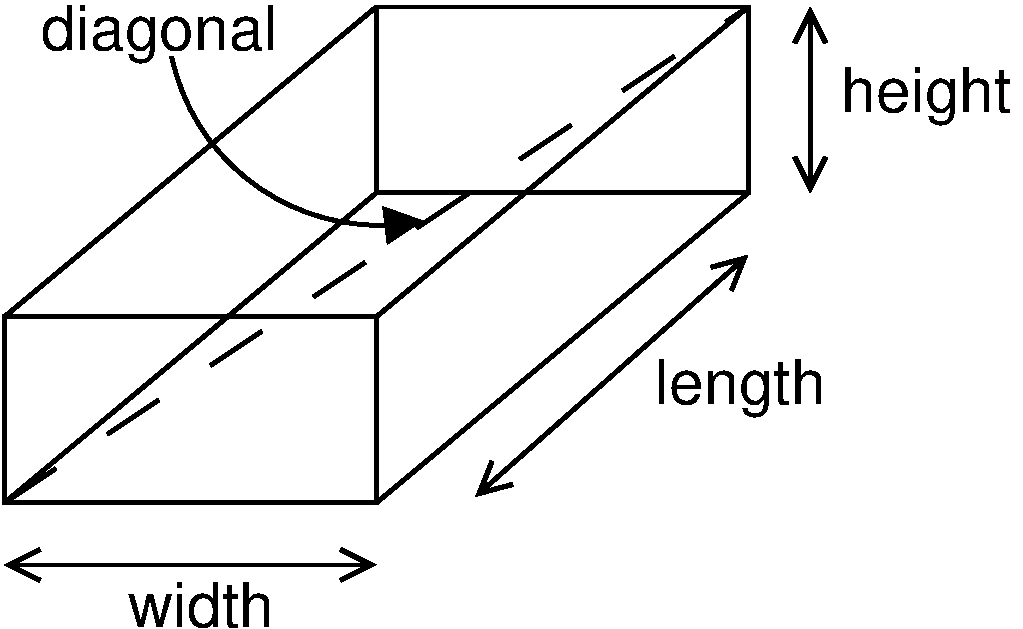
\includegraphics[scale=0.4]{figs/rectangular-prism.pdf}
\caption{Rectangular prism with length, width, height, and diagonal labeled.}
\label{fig.rectangular-prism}
\end{center}
\end{figure}

Write a program with these methods, all of which take the length, width, and height of the box as their three parameters and return a \java{double} result:

\begin{description}
\item \java{getVolume} \hfill \\ Returns the volume of the box.
\item \java{getSurfaceArea} \hfill \\ Returns the surface area of the box.
\item \java{getDiagonal} \hfill \\ Returns the diagonal distance of the box---the distance from the bottom left front corner of the box to the top right back corner.
\end{description}

The \java{main} method will prompt the user to enter the length, width, and height of a box and read them. It will then calculate and print the volume, surface area, and diagonal distance, properly labeled.

Here is an example of what the output might look like. Your program's output does not have to be identical to this, but it must reflect the same information:

\begin{stdout}
Enter length of box: 7
Enter width of box: 3.5
Enter height of box: 4

Volume: 98.00 cubic units
Surface area: 133.00 square units
Diagonal distance: 8.79 units
\end{stdout}

\end{exercise}

\begin{exercise}
The {\em Pythagorean distance} between points $(x_1, y_1)$ and $(x_2, y_2)$ is calculated as $\sqrt {(x_1-x_2)^2 + (y_1-y_2)^2}$. The code to find the Pythagorean distance is in the {\em Think Java 2nd Edition} book. Take the code from the book---or write it yourself---as a method named \java{distance} that takes four parameters (the coordinates of the two points) and returns the Pythagorean distance between those points. All the parameters and the return value are \java{double}.

Another way to measure the distance between two points is the ``city block'' distance: the sum of the absolute $x$ distance plus the absolute $y$ distance:
\begin{equation*}
|x_1 - x_2| + |y_1 - y_2|
\end{equation*}

For example, the city block distance from (1.5, 7) to (5, 2) is 8.5---the $x$ distance is 3.5 ($|1.5 - 5|$) and the $y$ distance is five ($|7 - 2|$).

Write a method named \java{cityBlockDistance} that takes the coordinates of the two points and returns the city block distance between them. All the parameters and the return value are \java{double}. {\em Hint:} Use \java{Math.abs} to calculate absolute value.

The \java{main} method will prompt the user to enter the coordinates; it will then calculate the Pythagorean distance using the \java{distance} method and print the returned result. Finally, \java{main} will call the \java{cityBlockDistance} method to calculate the city block distance and then print the returned result.
\end{exercise}

\begin{exercise}
The Pythagorean and city block distances are fine for a two-dimensional grid, but when you want to find the distance between two points on the spherical earth, you don't use a straight line. Instead, you calculate the {\bf great circle distance} from the latitude and longitude of the points.

Here is the formula where $r$ is the radius of earth in kilometers (6371.009), the first point's latitude and longitude are $lat_1$, $lon_1$ and the second point's latitude and longitude are  $lat_2$, $lon_2$:

\begin{equation*}
d = r\cdot cos^{-1}(sin(lat_1)\cdot sin(lat_2) + cos(lat_1)\cdot cos(lat_2)\cdot cos(lon_1 - lon_2))
\end{equation*}

{\bf Important!} The latitude and longitude in this formula are measured in {\em radians}, not degrees.

Write a method named \java{greatCircleDistance} which takes the latitude and longitude of two points {\em in degrees} as its four parameters and returns the great circle distance, which will be in kilometers.

You will also write a method named \java{kmToMiles} which takes as its single parameter a number of kilometers and returns the equivalent number of miles by multiplying by 0.621371.

Here are the latitude and longitude (in degrees) of several cities:
\begin{itemize}
\item San Jos\'e, California, USA: 37.333, -121.9
\item Los Angeles, California, USA: 34.05, -118.25
\item Seoul, South Korea: 37.56, 126.99
\item Vienna, Austria: 48.2, 16.367
\end{itemize}

Use this information to write the \java{main} method, which will calculate and print, properly labeled, the distance from San Jos\'e to Los Angeles and the distance from Seoul to Vienna. Print the distances in both kilometers and miles.

Here is the expected output:

\begin{stdout}
Distance from San Jose to Los Angeles: 492 km (306 miles)
Distance from Seoul to Vienna: 8277 km (5143 miles)
\end{stdout}

\end{exercise}



\chapter{Conditionals and Logic}

\begin{exercise}
Here is a table of wavelength ranges associated with the colors of visible light.

\renewcommand{\arraystretch}{1.5}  % put padding in array cells
\begin{tabular}{|l|l|l|r|}
\hline
{\bf Wavelength $\lambda$  in nm} & {\bf Color}\\ \hline
$0 < \lambda < 380$ & Ultraviolet \\ \hline
$380 \leq \lambda < 450$ & Violet \\ \hline
$450 \leq \lambda < 485$ & Blue \\ \hline
$485 \leq \lambda < 500$ & Cyan \\ \hline
$500 \leq \lambda < 565$ & Green \\ \hline
$565 \leq \lambda < 590$ & Yellow \\ \hline
$590 \leq \lambda < 625$ & Orange \\ \hline
$625 \leq \lambda < 700$ & Red \\ \hline
$700 \leq \lambda \leq 1000$ & Infrared \\ \hline
\end{tabular}

\renewcommand{\arraystretch}{1.0} % reset to no padding

Write a program that prompts the user for the wavelength of light and prints the corresponding color. If the value is less than or equal to zero or greater than 1000, print an error that tells what the correct range should be. Using an if-else chain is probably the best way to approach this exercise.
\end{exercise}

\begin{exercise}
Write a program that prompts the user for what percent of their maximum heart rate they achieved during an exercise session. The program will then describe the level of exercise they had:

\begin{tabular}{|l|l|l|r|}
\hline
{\bf \% {\em p} of maximum heart rate} & {\bf Description}\\ \hline
$0 < p < 50$ & Extremely light \\ \hline
$50 \leq p < 60$ & Very light \\ \hline
$60 \leq p < 70$ & Light \\ \hline
$70 \leq p < 80$ & Moderate \\ \hline
$80 \leq p < 90$ & Hard \\ \hline
$90 \leq p < 100$ & Maximumm \\ \hline
\end{tabular}

If the percentage entered is less than zero or more than 100, print an appropriate error message. Here is what the program output might look like for several runs of the program:

\begin{stdout}
What percent of your max heart rate did you reach? 72.8    
Your exercise session was: Moderate

What percent of your max heart rate did you reach? 92 
Your exercise session was: Maximum

What percent of your max heart rate did you reach? 102.6
Percent must be from 0 to 100.
\end{stdout}

\end{exercise}

\begin{exercise}
Here is a table that gives ticket prices for a movie theater. The price depends on the day of week, time of day, and age of the customer.

\renewcommand{\arraystretch}{1.5}  % put padding in array cells

\begin{tabular}{|l|l|l|r|}
\hline
Day & Time & Age & Price \\ \hline
Mon--Fri & Before 2 p.m. & All & \$5.00 \\ \cline {2-4}
& After 2 p.m. & Teen/Adult & \$6.00 \\
& & Child/Senior & \$4.50\\ \hline
Sat--Sun & Before 1 p.m. & Teen/Adult & \$6.50 \\
& & Child/Senior & \$5.25 \\ \cline{2-4}
& After 1 p.m. & Teen/Adult & \$8.00 \\
& & Child/Senior & \$5.50 \\ \hline
\end{tabular}

\renewcommand{\arraystretch}{1.0} % reset to no padding

Write a program that asks the user for:
\begin{itemize}
\item The day of the week, where 1 stands for Monday and 7 stands for Sunday
\item The time of day as an hour from 0 (midnight) to 23 (11:00 p.m.)
\item The customer's age. If a customer's age is from 13 to 64 (inclusive), they are a ``Teen/Adult''. Everyone else is a ``Child/Senior''.
\end{itemize}

The program then prints the ticket price for the customer. {\em Hint:} To make your code easier to read, write a method named \java{isTeenAdult} that takes the customer's age as its parameter and returns a \java{boolean} \java{true} if the age is from 13 to 64 (inclusive), \java{false} otherwise.

Do not allow the user to enter a day outside the range 1-7, an hour outside the range 0-23, or an age less than zero.

Using nested if-else statements is probably your best approach to this exercise.
\end{exercise}

\begin{exercise}
Write a program that prompts the user for a number in the range 1-12 and returns the number of days of that month. If the month is 2 (February) print that the month has 28 days in a normal year and 29 in a leap year. Be sure to validate the input.  Here is what the output from running the program several times might look like:

\begin{stdout}
Enter a month number (1-12): 3
Month number 3 has 31 days.

Enter a month number (1-12): 14
Invalid month; must be from 1 to 12.

Enter a month number (1-12): 2
Month number 2 has 28 days in a normal year
and 29 days in a leap year.
\end{stdout}

{\em Hint}: Use a \java{switch} statement to set a variable with the number of days in the month. Then, use an \java{if} statement to determine whether the month is February or not and print the appropriate output. Do {\em not} put the \java{System.out.println} inside the \java{switch} statement---that would lead to unnecessarily duplicated code.

\end{exercise}

\begin{exercise}
One phone messaging plan has a base cost of \$9.50 per month that includes 60 messages. You pay 4.5 cents for each message over 60 messages sent. The other messaging plan has a base cost of \$8.75 per month that includes 50 messages. You pay 5.2 cents for each message over 50 messages sent.

Write a program that will:

\begin{enumerate}
\item Ask the user for number of messages sent (integer).
\item Calculate and display the cost for the first plan.
\item Calculate and display the cost for the second plan.
\item Tell which plan is cheaper. The amounts for the two plans will never be exactly equal when the units are integers, although they may appear to be when rounded to two decimal places.
\end{enumerate}

Your program will use a method named \java{calculateCost} that returns the cost of a plan based on four parameters:
\begin{itemize}
\item The number of messages sent
\item The base cost per month
\item The number of messages included in the base cost (the ``base limit'')
\item The cost per message when you go over the base limit
\end{itemize}

Here are the results of running the program several times. Your output does not have to look exactly like this, but it must reflect the same information. All monetary amounts must be displayed with two digits after the decimal point.

\begin{stdout}
Enter number of messages: 40
Cost for plan one: $9.50
Cost for plan two: $8.75
Plan two is cheaper.

Enter number of messages: 80
Cost for plan one: $10.40
Cost for plan two: $10.31
Plan two is cheaper.

Enter number of messages: 150
Cost for plan one: $13.55
Cost for plan two: $13.95
Plan one is cheaper.
\end{stdout}

\end{exercise}

\begin{exercise}
This code fragment contains unnecessary condition tests:

\begin{code}
double bonus = 3.50;
if (hours < 10) {
    bonus = 0.50;
} else if (hours >= 10 && hours < 20) {
    bonus = 1.25;
} else if (hours >= 20 && hours < 40) {
    bonus = 2.25;
}
\end{code}

It can be rewritten like this:

\begin{code}
double bonus = 3.50;
if (hours < 10) {
    bonus = 0.50;
} else if (hours < 20) {
    bonus = 1.25;
} else if (hours < 40) {
    bonus = 2.25;
}
\end{code}

Why is it possible to eliminate the first condition before the \java{&&}? 

Now consider this code:

\begin{code}
double bonus = 3.50;
if (hours < 10) {
    bonus = 0.50;
}
if (hours >= 10 && hours < 20) {
    bonus = 1.25;
}
if (hours >= 20 && hours < 40) {
    bonus = 2.25;
}
\end{code}

Is it possible to eliminate the condition before the \java{&&} in this code? If so, why? If not, why not?
\end{exercise}

\begin{exercise}
Here is a program that asks a user for their age in years, tells the user their approximate age in days, and gives them a discount based on how old they are:

\begin{trinket}{DuplicatedCode.java}
import java.util.Scanner;

public class DuplicatedCode {

    public static void main(String[] args) {
        Scanner in = new Scanner(System.in);
        System.out.print("Enter your age in years: ");
        if (in.hasNextInt()) {
            int years = in.nextInt();
            int days = years * 365;
            double discount = 0.0;
            if (years > 0 && years < 18) {
                System.out.printf("That is about %d days.\n",
                    days);
                discount = years * 0.10;
                System.out.printf("Your discount is $%.2f\n",
                    discount);
            } else if (years < 21) {
                System.out.printf("That is about %d days.\n",
                    days);
                discount = years * 0.15;
                System.out.printf("Your discount is $%.2f\n",
                    discount);
            } else if (years < 65) {
                System.out.printf("That is about %d days.\n",
                    days);
                discount = years * 0.25;
                System.out.printf("Your discount is $%.2f\n",
                    discount);
            } else {
                System.out.printf("That is about %d days.\n",
                    days);
                discount = years * 0.40;
                System.out.printf("Your discount is $%.2f\n",
                    discount);
            }
        } else {
            System.out.println("Age must be numeric.");
        }
    }
}
\end{trinket}

The code works, but there is a lot of code that is repeated unnecessarily. Rewrite the code so that the code that prints the days and the code that prints the discount each appear only once in the program. Can you explain a general rule that tells when and how this sort of duplication can be eliminated?
     
\end{exercise}

\begin{exercise}
In the dice game called ```craps,'' the first phase of the game begins with a player rolling two dice.
If the total is 7 or 11, the player wins. If the total is 2, 3, or 12, the player loses. If the total is another number (4, 5, 6, 8, 9, or 10), that number is called the player's ``point,'' and the game enters its second phase, which we will not discuss here.

Write a program that simulates the first phase of the game by randomly rolling two dice and displaying the result.

Here is what the output from running the programs several times might look like:

\begin{stdout}
You rolled 3 and 5 - your point is 8.

You rolled 1 and 1 - you lose, sorry.

You rolled 3 and 4 - you win!
\end{stdout}

One difficulty of testing a program like this is that you have to wait for all combinations of dice to come up, but, since this is a random process, you could be waiting for a very long time. In order to test the program more easily, add code that lets you input the numbers for the dice directly:

\begin{code}
int die1 = // your java code to generate random number
int die2 = // your java code to generate random number
/* --- TESTING --- */
System.out.print("TEST - Enter values for dice: ");
die1 = in.nextInt(); // where "in" is your Scanner
die2 = in.nextInt();
in.nextLine(); // clear buffer in advance of String input
/* --- TESTING --- */
\end{code}

Your program output now looks like this when the program is run twice:

\begin{stdout}
TEST- Enter values for dice: 3 7
You rolled 3 and 7 - your point is 10.

TEST - Enter values for dice: 6 5
You rolled 6 and 5 - you win!
\end{stdout}

Remember to remove your testing code when you finish!

\end{exercise}

\begin{exercise}
In this exercise, you will modify the program from the preceding exercise to describe the results of the dice roll in words, using this table (adapted from \url{https://en.wikipedia.org/wiki/Craps}):

\begin{tabular}{|l|c|c|c|c|c|c|}
\hline
& 1 & 2 & 3 & 4 & 5 & 6 \\ \hline
1 & Snake Eyes & & & & & \\ \hline
2 & Ace Deuce & Hard Four & & & & \\ \hline
3 & Easy Four & Fever Five & Hard Six & & & \\ \hline
4 & Fever Five & Easy Six & Natural & Hard Eight & & \\ \hline
5 & Easy Six & Natural & Easy Eight & Nina & Hard Ten  & \\ \hline
6 & Natural & Easy Eight & Nina & Easy Ten & Yo-leven & Boxcars \\ \hline
\end{tabular}

Now the output from the program might look like this:

\begin{stdout}
You rolled 3 and 5: Easy Eight - your point is 8.

You rolled 1 and 1: Snake Eyes - you lose, sorry.

You rolled 3 and 4: Natural - you win!
\end{stdout}

{\em Hints}: For the ``Easy'' versus ``Hard'' combinations, if the dice values are equal, it's ``hard'' (in the sense of being more difficult to get that combination); all the others are considered ``easy.''

Do {\bf not} take the preceding program and blindly add code to it. Instead, carefully think through the new cases you must handle and the best way to handle them. (A 36-way \java{if} statement is definitely not your best choice.) Take time to plan it out! You might find that you have to re-structure your code to some degree to add this new feature. That's OK---that happens all the time when programming.

\end{exercise}


\chapter{Loops and Strings}

\section{The \java{do}-\java{while} Loop}
The following section is \copyright Alan Downey and Chris Mayfield, and is material that was originally in {\it Think Java}, but later removed. I think it's an important topic, so I am including it, slightly modified, here.

\index{pretest loop}
\index{loop!pretest}

The \java{while} and \java{for} statements are {\bf pretest loops}; that is, they test the condition first and at the beginning of each pass through the loop.

\index{posttest loop}
\index{loop!posttest}
\index{do-while}

Java also provides a {\bf posttest loop}: the \java{do}-\java{while} statement.
This type of loop is useful when you need to run the body of the loop at least once.

%NOTE: can we find an example that's better using do-while than using while-break?

For example, you can use a \java{do}-\java{while} loop to keep reading input until it's valid:

\begin{code}
Scanner in = new Scanner(System.in);
boolean okay;
do {
    System.out.print("Enter a number: ");
    if (in.hasNextDouble()) {
        okay = true;
    } else {
        okay = false;
        String word = in.next();
        System.err.println(word + " is not a number");
    }
} while (!okay);
double x = in.nextDouble();
\end{code}

Although this code looks complicated, it is essentially only three steps:

\begin{enumerate}
\item Display a prompt.
\item Check the input; if invalid, display an error and start over.
\item Read the input.
\end{enumerate}

\index{System.err}

The code uses a flag variable, \java{okay}, to indicate whether we need to repeat the loop body.
If \java{hasNextDouble()} returns \java{false}, we consume the invalid input by calling \java{next()}.
We then display an error message via \java{System.err}.
The loop terminates when \java{hasNextDouble()} return \java{true}.

Again, the important difference between \java{while} and \java{do}-\java{while} is this: In a \java{while} loop, the test happens {\em before} the loop body is executed. If the condition evaluates to \java{false}, the loop body doesn't get executed.

In a \java{do}-\java{while} loop, the loop body is always executed at least once, and only then is the condition evaluated. This turns out to be a good choice for validating input, because you must get the user's input before you can determine whether it's valid or not.

\section{Pre vs. Post Increment and Decrement}

\index{increment!pre vs. post}
\index{decrement!pre vs. post}

The book discusses the increment \java{++} and decrement \java{--} operators, which increase or decrease a variable's value by one.

You can put these operators before or after a variable name. For example, in this code fragment:

\begin{code}
int n = 47;
n++; // n post-increment to 48
++n; // n pre-increment to 49
n--; // n post-decrement to 48
--n; // n pre-decrement to 47
\end{code}

When a variable is all by itself, there is no difference between the operator before or after the variable. However, you may see people using these operators inside an expression, and then there is a very big difference.

Consider this code fragment:

\begin{code}
int n = 47;
int result = n++;
System.out.println("result is now " + n);
\end{code}

Because this is a post-increment, Java access the value of \java{n} and assigns it to \java{result}, and {\em then} adds one to \java{n}. It's as if we wrote it this way:

\begin{code}
int n = 47;
int result = n;
n = n + 1; // increment after assignment
System.out.println("result is now " + result);
\end{code}

If we place the \java{++} {\em before} the variable (a pre-increment):

\begin{code}
int n = 47;
int result = ++n;
System.out.println("result is now " + result);
\end{code}

Java will increment \java{n} {\em before} it assigns the value to \java{result}; it's as if we had written:

\begin{code}
int n = 47;
n = n + 1; // increment before assignment
int result = n;
System.out.println("result is now " + result);
\end{code}

While the following is not something you should do in your programs, you may see other people coding this way, and you'll need to understand it:

\begin{code}
int a = 7;
int b = 11;
int c = a++ * --b;
\end{code}

Here's the trick. First, find all the pre-increments and pre-decrements and evaluate them before the expression:

\begin{code}
int a = 7;
int b = 11;
b = b - 1; // do the pre-decrement
int c = a++ * b;
\end{code}

Then, find all the post-increments and post-decrements and evaluate them after the expression:

\begin{code}
int a = 7;
int b = 11;
b = b - 1;
int c = a * b;
a = a + 1;
\end{code}

Now there are no more increment and decrement operators, and you have just ``plain Java expressions,'' with the result being \java{c} being assigned \java{66}.

\section{Compound Assignment}
\index{compound assignment}
\index{assignment!compound}
The book mentions that you can increment a variable by two in this way:

\begin{code}
int n = 12;
n += 2; // same as n = n + 2;
\end{code}

I read this expression as ``\java{n} plus and becomes two.''

In fact, in any expression where the variable on the left side of the assignment operator is the same as the first variable on the right hand side, you can use this shortcut:

\begin{tabular}{|l|l|}
\hline
{\bf This:} & {\bf is the same as:} \\ \hline
\java{n += 2;} & \java{n = n + 2;} \\ \hline
\java{n -= 3;} & \java{n = n - 3;} \\ \hline
\java{n *= 4;} & \java{n = n * 4;} \\ \hline
\java{n /= 5;} & \java{n = n / 5;} \\ \hline
\java{n \%= 6;} & \java{n = n \% 6;} \\ \hline
\end{tabular}

You can use compound assignment in more complex expressions:
\java{n += m * 5;} is equivalent to \java{n = n + (m * 5);} However, you can {\em not} use it if the left-hand variable is part of a parenthesized expression. \java{n = (n + 7) * 3;} cannot be simplifed using compound assignment.

\section{Exercises}

\begin{exercise}
Write a program that asks the user for a starting amount of money, an annual interest rate as a percent, and a number of years. Use this information to print a table that shows the balance with accumulated compound interest. Use a \java{for} loop. Here is what your output might look like:

\begin{stdout}
Enter starting amount: $100
Enter annual percent interest: 5.3
Enter number of years: 4
Year  Balance
0     $100.00
1     $105.30
2     $110.88
3     $116.76
4     $122.95
\end{stdout}

\end{exercise}
\begin{exercise}
When you go to the store, the clerk doesn't know in advance how many items you want to buy. Instead, they keep totaling the items until they see one of those plastic dividers to indicate that your order is complete.

\index{sentinel value}
\index{value!sentinel}
Write a program that repeatedly asks the user for the price of an item until they enter a zero for the price. This is the digital equivalent of the plastic divider. Its technical name is a {\em sentintel value}. As the user enters prices, keep track of the total number of items and sum of the prices.  After encountering the sentinel value, your program will print the number of items purchased, the subtotal, the tax (at a rate of 6.5\%), and the grand total. Here is what the program might look like. Note that it does not allow (or count) negative prices. {\em Hint}: Use a \java{while} loop.

\begin{stdout}
Enter price, or 0 when finished: $3.50    
Enter price, or 0 when finished: $-2
Prices can not be negative.
Enter price, or 0 when finished: $5.99
Enter price, or 0 when finished: $4.83
Enter price, or 0 when finished: $0

Number of items: 3
Subtotal:  $   14.32
Tax:       $    0.93
Total:     $   15.25
\end{stdout}
\end{exercise}


\begin{exercise}
Write a program that repeatedly asks the user to enter a sentence (until they press only ENTER). For each sentence, tell how many vowels, consonants, digits, and ``other'' characters are in the sentence.  For this exercise, presume that the letter ``y'' is a vowel. Continue asking for sentences the user presses only the ENTER key for input. When that happens, the \java{String} that you read will equal the empty string \java{""}. You can test this condition to end the loop.

Sample output:

\begin{stdout}
Input a sentence (just ENTER to quit): 4 score & 7 years ago.
Vowels:   7  Consonants:  6
Digits:   2  Others:      7

Input a sentence (just ENTER to quit): 2*x=17
Vowels:   0  Consonants:  1
Digits:   3  Others:      2

Input a sentence (just ENTER to quit): The Quick Brown Fox
Vowels:   5  Consonants: 11
Digits:   0  Others:      3

Input a sentence (just ENTER to quit):
\end{stdout}

{\em Hint}: Make \java{String} variables with contents such as \java{"aeiouy"}, \java{"bcdfghjklmnpqrstvwxz"}, etc. and use \java{indexOf} to determine whether a character belongs to that group of characters.

\end{exercise}

\begin{exercise}
Write a method called \java{switchOrder}, which takes a \java{String} parameter with a person's name in the form \java{"first middle last"} and returns the name in the form \java{"last, first middle"}.  Your code should work for people with only a single name, people with no middle name, and people with several middle names.
Use a \java{while} loop with the \java{indexOf} and \java{substring} methods to do this exercise. (You could do it more easily with the \java{lastIndexOf} method, but we want you to get practice using loops.)

Write a \java{main} method that uses a \java{while} loop to repeatedly ask the user for a name and then calls the \java{switchOrder} method and prints the result. Repeat until the user presses just ENTER. Here is some sample output:

\begin{stdout}
Input a name (just ENTER to quit): Grace Murray Hopper
Hopper, Grace Murray

Input a name (just ENTER to quit): Donald Knuth   
Knuth, Donald

Input a name (just ENTER to quit): Prince
Prince

Input a name (just ENTER to quit): C. Anthony Richard Hoare
Hoare, C. Anthony Richard

Input a name (just ENTER to quit): 
\end{stdout}

\end{exercise}

\begin{exercise}
Write a program named{\it PhoneWord.java} that prompts the user for a ``phone word,'' an alphabetic mnemonic for a phone number. Then, print out the phone number corresponding to that sequence.

Here is how your program must translate letters to numbers:

\begin{tabular}{|l|l|}
\hline
ABC & 2 \\ \hline
DEF & 3 \\ \hline
GHI & 4 \\ \hline
JKL & 5 \\ \hline
MNO & 6 \\ \hline
PQRS & 7 \\ \hline
TUV & 8  \\ \hline
WXYZ & 9  \\ \hline
\end{tabular}

Keep digits as digits (see the second example output). Don't forget about zero!

You must accept letters in either upper or lower case. If the phone word translates to more than seven digits, keep only the first seven. If the phone word translates to fewer than seven digits, print an error message. Ignore any characters other than a letter or digit.

Here is an example of several runs of the program:

\begin{stdout}
Enter a phone word: warbler
The number is 9272537.

Enter a phone word: GOOD4U2
The number is 4663482.

Enter a phone word: OMG
Your phone word is not long enough for a phone number.

Enter a phone word: GREAT DEALS
The number is 4732833.

Enter a phone word: got-food?
The number is 4683663.

\end{stdout}

{\em Hint}: Do {\em not} check the input string to see if its length is greater than or equal to seven. The string 
\java{"C-A-T-S!"} is eight characters long, but there are only four letters, so it will not translate to a valid phone word.

Instead, convert all the letters in the string to digits, no matter how many or how few, and {\em then} check the length of the result to see if it is seven characters or more.

Extra challenge: Print the phone number with a hyphen; for example: 473-2833.

\end{exercise}

\begin{exercise}
Given an integer from 1 to 10 (inclusive), print a pattern of stars based on that number. Example:

\begin{stdout}
Enter number of rows: 4
*
**
***
****
\end{stdout}
\end{exercise}

\begin{exercise}
Given an integer from 1 to 10 (inclusive), print an inverted triangle of plus signs based on that number. Example:

\begin{stdout}
Enter number of rows: 6
+++++++++++
 +++++++++
  +++++++
   +++++
    +++
     +
\end{stdout}

{\em Hint}: make a table with the line number (starting at zero or one, but zero is probably better), the number of leading spaces you will need on the line, and the number of plus signs. Then figure out the mathematical relationships between the line number and the other two values. They will be linear relationships.
\end{exercise}


\chapter{Arrays and References}

\section{Passing Arrays to Methods}

When you pass an array to a method, you are passing a {\em copy of the reference} to the array. Consider this code:

\begin{code}
import java.util.Arrays;

public static void main(String[] args) {
    double [] data = {4.0, 7.0, 2.5};
    squareArray(data);
    System.out.println(Arrays.toString(data));
}

public static void squareArray(double[] arr) {
    for (int i = 0; i < arr.length; i++) {
        arr[i] = arr[i] * arr[i];
    }
}
\end{code}

Figure~\ref{fig.passArray1} is what memory looks like upon entry to \java{squareArray}. Java does not copy the argument array's contents into the parameter. Instead, Java copies the {\em reference} to the argument \java{data} into the parameter \java{arr}.

\begin{figure}[!h]
\begin{center}
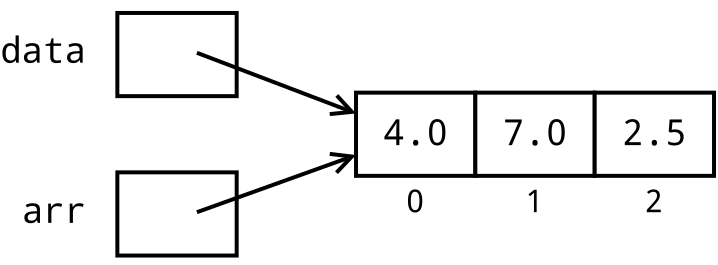
\includegraphics[scale=0.5]{figs/ch07/pass_to_array1.png}
\caption{Variable \java{arr} is a copy of the reference variable \java{data}}
\label{fig.passArray1}
\end{center}
\end{figure}

When the loop ends, the elements in the array have all changed, as show in Figure~\ref{fig.passArray2}.

\begin{figure}[!h]
\begin{center}
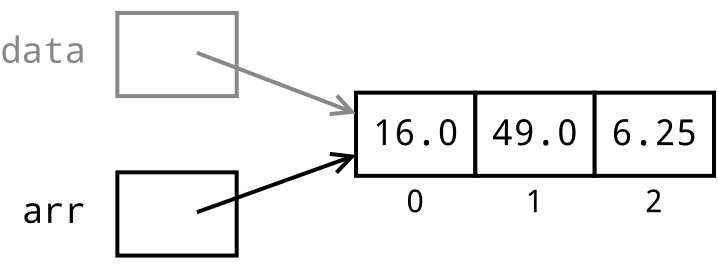
\includegraphics[scale=0.5]{figs/ch07/pass_to_array2.png}
\caption{\java{arr} refers to updated array contents}
\label{fig.passArray2}
\end{center}
\end{figure}

When method \java{squareArray} ends, its stack frame goes away and we are left with \java{data} referring to the changed array, as shown in Figure~\ref{fig.passArray3}.

\begin{figure}[!h]
\begin{center}
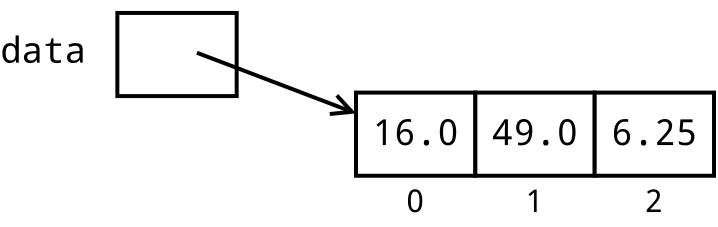
\includegraphics[scale=0.5]{figs/ch07/pass_to_array3.png}
\caption{Variable \java{data} refers to changed array contents}
\label{fig.passArray3}
\end{center}
\end{figure}

When you pass an array to a method, you get a copy of the {\em reference}. Your methods can modify the contents of the array via the reference.

Why does Java pass a copy of the reference instead of a copy of the contents? Because back when Java was invented, CPUs were slow and memory was limited. Copying the four- or eight-byte memory address of a thousand-element array is much faster than copying all thousand elements. That's the good news.

The bad news is that you can change an array's contents inadvertently. In the preceding example, once you call \java{squareArray}, your original data is gone. If you call \java{squareArray} again, you end up with the elements of the original array to the fourth power!

\section{Returning Arrays from Methods}

We're no longer working in a ``scarcity model,'' where every byte and microsecond is precious. Nowadays, CPUs are fast enough and memory plentiful enough that it makes sense to return a new array from a method, leaving the original untouched.

Consider this revised code, with line numbers for reference:

\begin{code}
 1 import java.util.Arrays;
 2
 3 public static void main(String[] args) {
 4     double [] data = {4.0, 7.0, 2.5};
 5     double [] squaredData = newSquareArray(data);
 6     System.out.println(Arrays.toString(data)); 
 7     System.out.println(Arrays.toString(squaredData));
 8 }
 9
10 public static double[] newSquareArray(double[] arr) {
11     double[] result = new double[arr.length];
12    
13     for (int i = 0; i < arr.length; i++) {
14         result[i] = arr[i] * arr[i];
15     }
16     return result;
17 }
\end{code}

Notice the return type in line 10: the method returns an array of \java{double}---the square brackets indicate an array.

When line 5 calls \java{newSquareArray}, line 11 creates a reference named \java{result} that refers to a new array with the same length as the original array. The loop changes the value in \java{result}, leaving the argument \java{arr} unmodified. Figure~\ref{fig.returnArray1} shows the memory diagram at the end of the loop.

\begin{figure}[!h]
\begin{center}
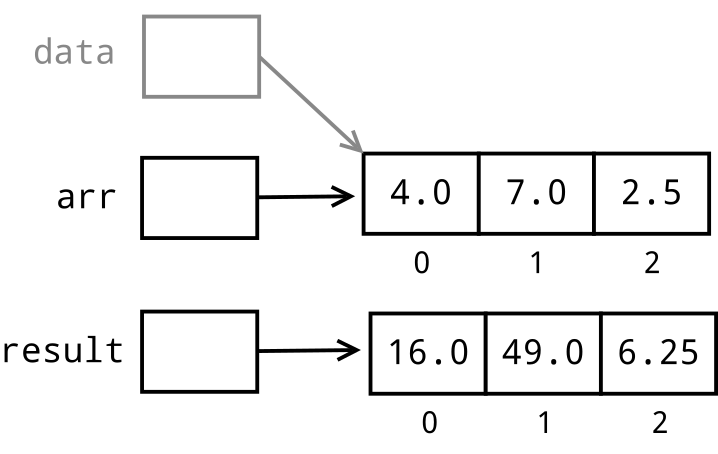
\includegraphics[scale=0.5]{figs/ch07/return_array1.png}
\caption{\java{arr} and \java{result} refer to different arrays}
\label{fig.returnArray1}
\end{center}
\end{figure}

In line 16, the method returns \java{result}, which, again, is a reference to the squared values. The return value is stored in \java{squaredData} on the left side of the assignment in line 5.  Figure~\ref{fig.returnArray2} shows the memory diagram after line 5.

\begin{figure}[!h]
\begin{center}
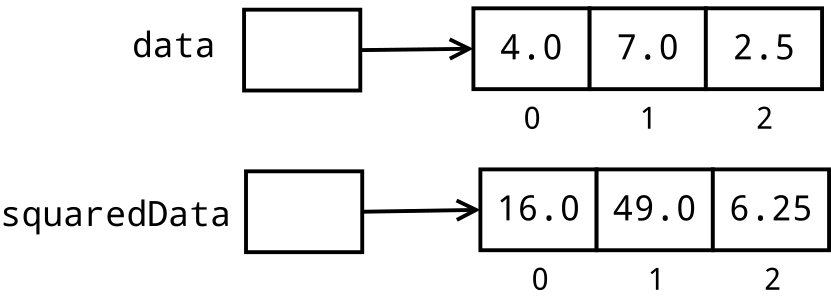
\includegraphics[scale=0.5]{figs/ch07/return_array2.png}
\caption{\java{data} and \java{squaredData} refer to different arrays}
\label{fig.returnArray2}
\end{center}
\end{figure}

So, which should you do? Update arrays in place (as in the first example) or return new arrays (as in the second example)?  There is a programming paradigm called {\em functional programming} that strongly prefers the second approach. From a functional programming standpoint, the ability to change an array in place is bad style at best and a dangerous source of programming errors at worst. In my opinion, and this is {\em only an opinion}, I agree with that viewpoint. As a guideline (not a rule), I suggest that you write your programs to return new arrays rather than modifying array arguments. However, if you are programming in an environment where memory is at a premium and programs run on slow processors, as can happen when you are programming embedded systems (\url{https://en.wikipedia.org/wiki/Embedded_system}), then saving space and time by modifying the array may be the better approach.

In the following exercises, you will be writing some methods that update an array in place and others that return a new array. This will let you practice both approaches.

\section{Exercises}

\begin{exercise}
Write methods named \java{getMax} and \java{getMin} that take an array of integers as their parameters and return the largest and smallest values in the array. Presume that the array has at least one element, and use a loop to traverse the elements.  {\em Hint}: Set the return value to the first element of the array before you enter the loop. This guarantees that your return value will be an element in the array.

Write a \java{main} method to test \java{getMax} and \java{getMin}. For example:

\begin{stdout}
Enter array length: 6
Enter 6 integers separated by spaces: 47 505 10 66 11 217
Minimum value: 10
Maximum value: 505
\end{stdout}

\end{exercise}

\begin{exercise}
The {\em Think Java} book has code to generate a histogram of scores from 0-100. In this exercise, you will generalize this to a method that accepts an array of integers as its parameter and displays the histogram.  The method is declared as:

\begin{code}
public static void displayCounts(int[] values,
     int categories, int min, int max)
\end{code}

\begin{itemize}
\item \java{values} an array of integers with the values whose histogram you want
\item \java{categories} how many ``bars'' the histogram has
\item \java{min} the minimum value of the histogram categories
\item \java{max} the maximum value of the histogram categories
\end{itemize}

For example, given this array and these calls:

\begin{code}
int[] data =  {35, 37, 19, 45, 49, 68, 95, 7, 5, 82, 84};
displayCounts(data, 5, 0, 100);
System.out.println("-----------");

// use getMin and getMax methods from preceding exercise
displayCounts(data, 4, getMin(data), getMax(data));
\end{code}

Generates this output:

\begin{stdout}
0-19: 3
20-39: 2
40-59: 2
60-79: 1
80-100: 3
-----------
5-26: 3
27-48: 2
49-70: 2
71-95: 4
\end{stdout}

You have to do some extra work to make sure that the maximum value is included in the output of the last category range. Notice, for example, in the first histogram, all the categories have a range of 20 except the last, which has a range of 21.
\end{exercise}

\begin{exercise}
\label{ex:standardize}
Write the following methods, each of which takes an array of \java{double} values as a parameter:

\begin{itemize}
\item The \java{mean} method returns the arithmetic mean (average) of the array elements.

\item The \java{stdev} method returns the standard deviation of the array elements, using this formula
\begin{equation*}
s = \sqrt {{n \sum{x_i} ^2 - \left(\sum{x_i}\right)^2} \over {n (n - 1)}}
\end{equation*}

where $n$ is the number of items in the array, $\sum{x_i} ^2$ is the sum of the squares of the individual items, and $\left(\sum{x_i}\right)^2$ is the square of the total of all the items in the array.

\item The \java{standardize} returns a new array of the values converted to {\em standard scores}. First, calculate the mean $m$ and standard deviation $s$ of the entries in the original array. Each entry in the result array will be \java{(arr[i] - m) / s}. This method must call the \java{mean} and \java{stdev} methods.

Write a \java{main} method to test the \java{standardize} method. For example, an array with values
\java{\{47.0, 11.0, 10.0, 66.0, 8.5\}} will generate these standard scores: \java{\{0.700, -0.662, -0.700, 1.418, -0.756\}} (to three decimal places). 

\end{itemize}
\end{exercise}

\begin{exercise}
\label{ex:stringReversal}

Unlike the string reversal method shown in {\em Think Java}, where a program built a new string that had its characters in the reverse order of the original, in this exercise you will write a \java{void} method named \java{reverseInPlace} that takes an array of integers as its parameter and reverses the order of the items in the array--in place. In other words, you won't create a new array; you will change the order of the items within the array itself.

Write a \java{main} method that will test the method by reversing and displaying:

\begin{enumerate}
\item An empty array with no elements
\item An array with one element
\item An array with an even number of elements (more than two elements)
\item An array with an odd number of elements (more than three elements)
\end{enumerate}

To make your job easier, you might want to create a ``helper method'' named \java{reverseAndDisplay} that prints the array, calls \java{reverseInPlace} and prints the array (which should now be reversed).
\end{exercise}

\begin{exercise}
\label{ex:vectors}

You can use an array of three \java{double} values to represent a {\em vector} in three-dimensional space. The first element represents the vector's $x$-component, the second its $y$ component, and the third its $z$ component, written as $(x, y, z)$. Write a program that has these methods, each of which takes two three-element arrays as parameters:
\begin{itemize}
\item \java{add}: Returns a vector (an array of length three) representing the sum of the parameters. The sum of $(x_1, y_1, z_1)$ and $(x_2, y_2, z_2)$ is the vector $(x_1 + x_2, y_1 + y_2, z_1 + z_2)$
\item \java{dotProduct}: Returns the {\em dot product} of the parameter vectors. The dot product of  $(x_1, y_1, z_1)$ and $(x_2, y_2, z_2)$ is calculated as $x_1\cdot x_2 + y_1\cdot y_2 + z_1\cdot z_2$ 
\item \java{distance}: Returns the distance between the vectors $(x_1, y_1, z_1)$ and $(x_2, y_2, z_2)$ using the formula $\sqrt{(x_1 - x_2)^2 + (y_1 - y_2)^2 + (z_1 - z_2)^2}$
\end{itemize}

The \java{main} method will ask the user to enter two vectors and then display the sum, dot product, and distance between the vectors. To avoid repetitious code, you might want to write a \java{getVector} method that has a prompt and a \java{Scanner} as its parameters. This method will prompt the user for the three vector components and return an array of three \java{double} values.

Here is an example of what the program might look like:

\begin{stdout}
Enter components of the first vector,
separated by spaces: 2 1.5 4.1
Enter components of the second vector,
separated by spaces: 7 3.5 1.2
Sum of vectors: (9.000, 5.000, 5.300)
Distance between vectors: 6.116
Dot product of vectors: 24.170
\end{stdout}

\end{exercise}

\begin{exercise}
In this exercise, you will find the correlation between the elements in two arrays of equal length.
Your program will ask the user for the number of entries in each array, read them in, and see how good a linear relationship they have to each other by calculating the {\em correlation coefficient}. This is a number that ranges from 1.0 (the two arrays are perfectly related to each other) to -1.0 (the arrays are perfectly inversely correlated to one another---as an example, think of the heights of the two ends of a seesaw in motion). A correlation of zero means the values in the two arrays have no linear relationship.

Write a method named \java{correlation} that takes two arrays of double and returns the correlation coefficient $r$ according to this formula, where $\bar x$ stands for the mean of $x$ and $\bar y$ stands for the mean of $y$.

\begin{equation*}
r = {{ \sum{( x_i - \bar x) (y_i - \bar y)}} \over {\sqrt { \sum{(x_i - \bar x)^2 \sum{(y_i -\bar y)^2} }}}}
\end{equation*}

This is the {\em classical formula} for correlation, and it requires you to have an array. The code will have to go through the arrays once to find the averages, and again to do the subtractions in the equation. There is a {\em computational formula} for correlation which can do the calculation without needing to store the numbers in an array, but that would defeat the purpose of giving you practice with arrays.

Here is an example of what the output might look like. The data are people's height in centimeters for the first array and their weight in kilograms for the second array.

\begin{stdout}
Enter number of elements in each array: 5
Enter the 5 elements in the first array: 178 176 160 180 186
Enter the 5 elements in the second array: 84.2 77.3 60 65.5 82.1
The correlation coefficient is 0.710.
\end{stdout}

\end{exercise}

\begin{exercise}
Write a method called \java{separate} which takes an array of integers as its argument and returns a new array that consists of all odd elements in the first array followed by all the even numbers in the first array, in the same relative order.

This method will require two passes (traversals) through the array.

Then, write a \java{main} method to test the \java{separate} method. Here is what it
might look like:

\begin{stdout}
Enter number of items in array: 6
Enter the items, separated by spaces: 10 47 11 66 5 98
Array with odd, then even elements: [47, 11, 5, 10, 66, 98]
\end{stdout}

You may use the \java{java.utils.Arrays.toString} method to print the result array. Make sure you test your program with an array that contains only odd numbers and again with only even numbers.

\end{exercise}



\chapter{Recursive Methods}

\section{Tail Recursion}

Let's take another look at the \java{factorial} method from the book and its stack frames in Figure~\ref{fig.factorial_stack}.

\begin{code}
public static int factorial(int n) {
    if (n == 0) {
        return 1;
    }
    int recurse = factorial(n - 1);
    int result = n * recurse;
    return result;
}
\end{code}

\begin{figure}[!htb]
\begin{center}
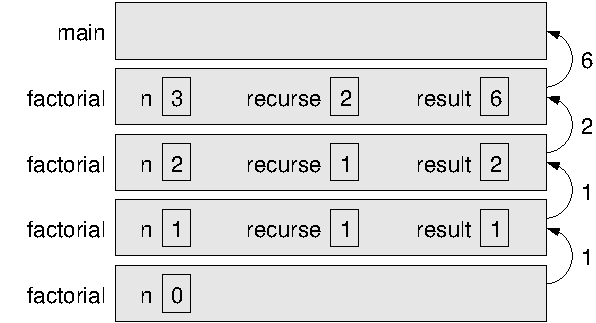
\includegraphics{figs/ch08/stack3.pdf}
\caption{Stack diagram for the \java{factorial} method.}
\label{fig.factorial_stack}
\end{center}
\end{figure}


The program can't calculate \java{factorial(3)} until it has figured out \java{factorial(2)}, which can't be calculated until \java{factorial(1)} is calculated, and so on.

This means that when the program gets to the base case, it has to return the result to the previous call, which has to return the result to {\em its} caller, passing results back up the call chain until the result is finally calculated. This process is indicated by the arrows in the diagram, and this is the process that tends to confuse people when they're learning about recursion.

On the other hand, look at \java{countdown} method and its stack frames in Figure~\ref{fig.countdown_stack}. 

\begin{code}
public static void countdown(int n) {
    if (n == 0) {
        System.out.println("Blastoff!");
    } else {
        System.out.println(n);
        countdown(n - 1);
    }
}
\end{code}

When the program hits the base case,  (\java{n == 0}) it's finished. There are no arrows in the diagram because there's no result to pass back to the previous caller; it's a \java{void} method.

\begin{figure}[!htb]
\begin{center}
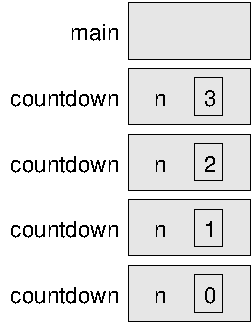
\includegraphics{figs/ch08/stack2.pdf}
\caption{Stack diagram for the \java{countdown} program.}
\label{fig.countdown_stack}
\end{center}
\end{figure}

This is why the book introduced recursion with the \java{countdown} method; it's conceptually simpler.

There is one other important difference between these two methods. In \java{countdown}, the recursive call is the very last thing that happens in the non-base case.  In \java{factorial}, the recursive call isn't the very last thing that happens. This is why the result has to be ``on hold'' until reaching the base case.

\index{tail recursion}
\index{recursion!tail}
When the recursive call is the very last thing that happens in the non-base case, the method is called a {\em tail recursive} method.

Even if you were to rewrite the \java{factorial} method in the following way, it would still {\em not} be tail recursive.

\begin{code}
public static int factorial(int n) {
    if (n == 0) {
        return 1;
    } else {
        return n * factorial(n - 1);
    }
}
\end{code}

In this version of the code, the recursive call to \java{factorial} still isn't the last thing that happens---the multiplication is the last operation.

Is it possible to write methods like \java{factorial} so that they use tail recursion? Yes, it is, by using something that I call the ``accumulator trick.'' We're going to write the method so that the accumulated result is one of the method parameters:

\begin{code}
public static int tailFactorial(int n, int result) {
    if (n == 0) {
        return result;
    } else {
        tailFactorial(n - 1, n * result);
    }
}
\end{code}

You call it like this:

\begin{code}
int fac3 = tailFactorial(3, 1); // initial value of result is 1
\end{code}

Let's see what happens when we call \java{tailFactorial(3, 1)}.

\vspace{-1ex}
\begin{quote}
\java{n} is 3 and \java{result} is 1. Since 3 is not 0, we call \java{tailFactorial(2, 3 * 1)}
\begin{quote}
\java{n} is 2 and \java{result} is 3. Since 2 is not 0, we call \java{tailFactorial(1, 2 * 3)}
\begin{quote}
\java{n} is 1 and \java{result} is 6. Since 1 is not 0, we call \java{tailFactorial(0, 6 * 1)}
\begin{quote}
\java{n} is 0 and \java{result} is 6. Since 0 {\em is} 0, we return the value of \java{result}, which is the correct answer: 6.
% without making any more recursive invocations.
\end{quote}
\end{quote}
\end{quote}
\end{quote}
\vspace{-1ex}

Once we hit the base case, we have the answer we want---it's passed all the way back up the chain.

Figure~\ref{fig.tail_recursive} shows the call stack for \java{tailFactorial}. You can think of the base case returning the accumulated result directly to the original caller.

\begin{figure}[!htb]
\begin{center}
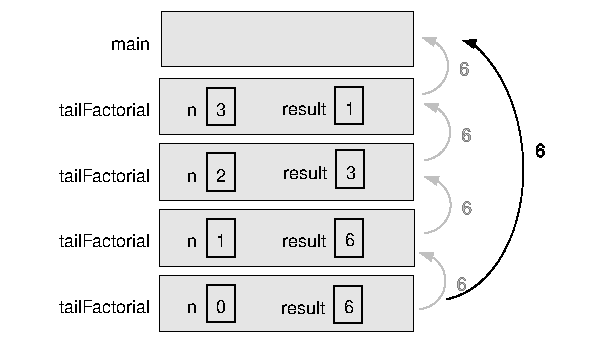
\includegraphics{figs/ch08/stack4.pdf}
\caption{Stack diagram for the \java{tailFactorial} program.}
\label{fig.tail_recursive}
\end{center}
\end{figure}

\index{tail call optimization}
\index{optimization!tail call} In fact, some languages, but {\em not} Java, do {\em tail call optimization}. Since all the necessary information is carried from stack frame to stack frame, these languages can optimize the code so that it re-uses the same stack frame over and over again. With this optimization, stack overflow cannot occur.

Even though Java doesn't do tail call optimization, you should still learn the ``accumulator trick.'' First, it's conceptually simpler: once you hit the base case, you've finished. Second, if you know how to write tail recursive methods in other languages that {\em do} optimize, you'll be in a position to take advantage of it.

\section{Overloaded Methods}
In the \java{tailFactorial} example, the user has to provide the number whose factorial they want as well as the starting value for the accumulator. We could make life easier for our users by providing a one-parameter \java{factorial} method for the convenience of our users:

\begin{code}
public int factorial(int n) {
    // Provide the result value
    // for the user's convenience
    return tailFactorial(n, 1); 
}
\end{code}

They would then be able to write code like this:

\begin{code}
int answer = factorial(7);
\end{code}

In this example, we have two different method names: \java{tailFactorial} and \java{factorial}. Many programming languages {\em require} you to have different names for all your methods. Java, however, is one of those languages which allow you to have multiple methods with the same name---as long as they have a different number and/or type of their parameters. This is called an {\em overloaded method}.

While overloading methods indiscriminately can lead to code that is difficult to read and maintain, overloading does have its place. For example, if you look at the documentation for the \java{Math} class at \url{https://docs.oracle.com/en/java/javase/16/docs/api/java.base/java/lang/Math.html}, you will see that the \java{Math.abs} method is overloaded to accept different data types.

We could write the preceding example to use overloading.

\begin{code}
 1 public static int factorial(int n, int result) {
 2     if (n == 0) {
 3         return result;
 4     } else {
 5         factorial(n - 1, n * result);
 6     }
 7 }
 8 
 9 public static int factorial(int n) {
10     factorial(n, 1);
11 }
12 
13 public static void main(String[] args) {
14     int answer = factorial(7);
15 }
\end{code}

When Java encounters the call on line 14, it sees there is only one parameter and calls the corresponding \java{factorial} method on line 9. When it gets to the call on line 10, it sees there are two parameters and calls the corresponding \java{factorial} method on line 1. The call on line 5 has two parameters, which means it is a recursive call to the method on line 1.

\section{Exercises}

\begin{exercise}
Find whether a \java{String} is a palindrome (the same forward and backwards, such as ``radar'' or ``racecar''). Write an \java{isPalindrome} method with this header:

\begin{code}
public static boolean isPalindrome(String s, int start, int end) 
\end{code}

where \java{s} is the string you are testing, \java{start} is the starting index in the string, and \java{end} is the ending string.

If the characters at the \java{start} and \java{end} position are not identical, return \java{false}; it's not a palindrome. Otherwise, \java{return} the result of a recursive call to \java{isPalindrome}, adding one to the \java{start} position and subtracting one from the \java{end} position.

The base case occurs when the \java{start} and \java{end} position are the same, which happens for words like ``radar``, or when \java{start} becomes greater than \java{end}, which happens for words like ``anna''. If you reach the base case, return \java{true}.

As described here, this is a naturally tail recursive process. Either it fails on a mismatch, or you hit the base case and you've finished.

\end{exercise}


\begin{exercise}
Write a tail recursive method to find the sum of an array of integers. To use the accumulator trick in this method, you'll need to keep track of {\em two} things: one for the current index into the array and another for the accumulated sum, which starts at 0. The base case occurs when the index equals the array length; at that point you have the result in the accumulated sum. The method header might look like this:

\begin{code}
public static int sum(int[] arr, int index, int sum)
\end{code}

You would call it like this:

\begin{code}
int[] data = {10, 47, 66, 11};
int total = sum(data, 0, 0);
\end{code}

\end{exercise}

\begin{exercise}
Write a tail recursive method to find the {\em n}th Fibonacci number. To use the accumulator trick in this method, you'll need to keep track of which Fibonacci number you're working on ({\em hint}: it counts down), the current result, and the previous result. The method header might look like this:

\begin{code}
public static int fibonacci(int n, int result, int previous)
\end{code}

The base case occurs when \java{n} is 1 or 2, in which case you return 1.

You would call it like this:

\begin{code}
// Find the twelfth Fibonacci number
int answer = fibonacci(10, 1, 1); // should be 55
\end{code}

\end{exercise}

\begin{exercise}
In order to make your methods more friendly to users, use method overloading to implement these methods for the preceding exercises:

\begin{itemize}
\item \java{public static boolean isPalindrome(String s)}
\item \java{public static int sum(int[] arr)}
\item \java{public static int fibonacci(int n)}
\end{itemize}
\end{exercise}


%~ \part{Object-Oriented Programming}

\chapter{Immutable Objects}

\section{What Does Immutability Mean?}

Many people read the statement that ``Java \java{String}s are immutable'', and then write code like this:

\begin{code}
String metal;
metal = "lead";
metal = "gold";
\end{code}

and ask ``Didn't that just change the string?''  No, that code does not change lead into gold.

Let's take a look at a memory diagram after the first assignment. \java{metal} is a {\em reference} to an area of memory (called the {\bf heap}) where the string \java{"lead"} has been allocated.

\begin{figure}[!h]
\begin{center}
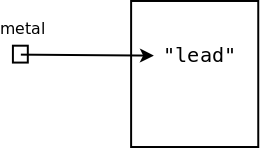
\includegraphics[scale=0.4]{figs/heap1.png}
\caption{Reference to a String on the heap}
\label{fig.heap1}
\end{center}
\end{figure}

After the second assignment, the {\em reference} has changed to refer to another portion of the heap that contains the string \java{"gold"}. The string \java{"lead"} is still on the heap, unmodified. It's just that nobody is referring to it any longer.

\begin{figure}[!h]
\begin{center}
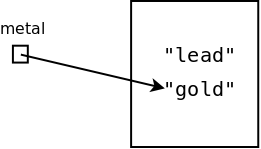
\includegraphics[scale=0.4]{figs/heap2.png}
\caption{Reference to a second String on the heap}
\label{fig.heap2}
\end{center}
\end{figure}

What would ``changing the string'' look like? In some languages, a string is treated as if it were an array of characters, and you could write code like this:

\begin{code}
metal = "gold";
metal[0] = 's'; // change first letter to 's'
\end{code}

Java won't let you do that because the string itself, which is out there on the heap, cannot be modified.

\begin{figure}[!h]
\begin{center}
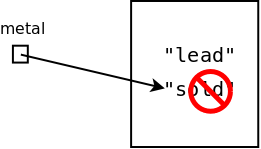
\includegraphics[scale=0.4]{figs/bad_heap.png}
\caption{Non-Java modified string (illegal in Java)}
\label{fig.bad.heap}
\end{center}
\end{figure}

But there's nothing to stop you from creating a brand new \java{String} on the heap and changing the value of \java{metal} to refer to that new \java{String}, as shown in Figure~\ref{fig.heap3}:

\begin{code}
metal = "s" + metal.substring(1, 4);
\end{code}

\begin{figure}[!h]
\begin{center}
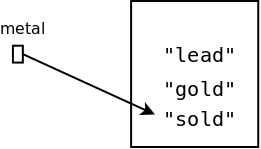
\includegraphics[scale=0.4]{figs/heap3.png}
\caption{Reference to a newly created String on the heap}
\label{fig.heap3}
\end{center}
\end{figure}

\clearpage

\section{Generalizing and the \java{Scanner} Class}

The {\em Think Java} book's subtitle is ``How to Think Like a Computer Scientist,'' and in that spirit, places more emphasis on the concepts of computer science---developing and analyzing algorithms. In order to do this, the book deliberately avoids going into the minutiae of the Java language. At this point, however, we have to get into a detail of the \java{Scanner} class that comes up when you are generalizing and modularizing your code.

Whenever you generalize a method for doing input, do {\em not} create the \java{Scanner} inside the method. Instead, you must pass a \java{Scanner} object as one of the parameters.

Consider the following program that asks a user for two prices and calculates the percentage change:

\begin{code}
import java.util.Scanner;

public class RepeatedCode {
  public static void main(String[] args) {
    Scanner input = new Scanner(System.in);
    double originalPrice;
    do {
      System.out.print("Enter original price: ");
      originalPrice = input.nextDouble();
      if (originalPrice <= 0) {
        System.out.println("Price must be greater than zero.");
      }
    } while (originalPrice <= 0);
    
    double newPrice;
    do {
      System.out.print("Enter new price: ");
      newPrice = input.nextDouble();
      if (newPrice <= 0) {
        System.out.println("Price must be greater than zero.");
      }
    } while (newPrice <= 0);
    
    double pctChange = 100.0 *
      (newPrice - originalPrice) / originalPrice;
    System.out.printf("Price change: %.1f%%\n", pctChange);
  }
}
\end{code}

The code for the two inputs is identical except for the prompt (and the variable name). Here is a way to generalize that code by creating a method to get the input and having the input prompt as its parameter:

\begin{code}
import java.util.Scanner;

public class GeneralInput1 {
  
  public static double getPrice(String prompt) {
    Scanner input = new Scanner(System.in);
    double price;
    do {
      System.out.print(prompt);
      price = input.nextDouble();
      if (price <= 0) {
        System.out.println("Price must be greater than zero.");
      }
    } while (price <= 0);
    return price;
  }

    
  public static void main(String[] args) {
    double originalPrice = getPrice("Enter original price: ");
    double newPrice = getPrice("Enter new price: ");
    double pctChange = 100.0 *
      (newPrice - originalPrice) / originalPrice;
    System.out.printf("Price change: %.1f%%\n", pctChange);
  }
}
\end{code}

This program works, but there's a trap hidden in it. Every time the code calls \java{getPrice}, a new \java{Scanner} is created, opening a new connection to the keyboard. This is inefficient, but not fatal---until someone tells you that you should always close an I/O device and you add the code \java{input.close();} between the end of the loop and the \java{return} statement.

Once the \java{input} is closed, its connection to the keyboard is broken {\em and cannot be re-opened}. Now, when you run the program, you get this result:

\begin{stdout}
Enter original price: 3.50
Enter new price: Exception in thread "main"
  java.util.NoSuchElementException
        at java.base/java.util.Scanner.throwFor(Scanner.java:937)
        at java.base/java.util.Scanner.next(Scanner.java:1594)
        at java.base/java.util.Scanner.nextDouble(Scanner.java:2564)
        at BadClose.getPrice(BadClose.java:10)
        at BadClose.main(BadClose.java:22)
\end{stdout}

In order to avoid the minor problem of creating multiple connections to the keyboard and the major problem of inadvertently closing the connection before you want to, your code must create the \java{Scanner} once, and once only. Here is code that solves the problem. It creates the \java{Scanner} once in \java{main}, closes it only once the end of \java{main}, and passes it as an additional argument to the \java{getPrice} method:

\begin{code}
import java.util.Scanner;

public class GeneralInput2 {
  
  public static double getPrice(Scanner in, String prompt) {
    double price;
    do {
      System.out.print(prompt);
      price = in.nextDouble();
      if (price <= 0) {
        System.out.println("Price must be greater than zero.");
      }
    } while (price <= 0);
    return price;
  }

    
  public static void main(String[] args) {
    Scanner input = new Scanner(System.in);
    double originalPrice = getPrice(input, "Enter original price: ");
    double newPrice = getPrice(input, "Enter new price: ");
    double pctChange = 100.0 *
      (newPrice - originalPrice) / originalPrice;
    System.out.printf("Price change: %.1f%%\n", pctChange);
    input.close();
  }
}
\end{code}

\section{Exercises}

\begin{exercise}
In this exercise, we will once again rewrite the ``dew point'' program. Prompt the user for the air temperature in degrees Celsius and the relative humidity as a percent, and calculate the dew point with this formula:

\begin{equation*}
dewPoint = temperature - {{100 - relHumidity} \over 5}
\end{equation*}

Generalize the code to use a method to get the temperature. This method should accept only numbers in the range -90 to 60 degrees Celsius, giving an error message if the temperature is out of range. (The range given here includes the lowest and highest recorded temperatures on earth.)

Write a method to get the relative humidity. This method should accept only numbers in the range 0 to 100, giving an error message if the relative humidity is out of range.

Here is what output might look like when the user enters several out-of-range values:

\begin{stdout}
Enter temperature in degrees C: 85
Value must be in range -90 to 60.
Enter temperature in degrees C: -100
Value must be in range -90 to 60.
Enter temperature in degrees C: 20
Enter relative humidity as a percent: -20
Value must be in range 0 to 100.
Enter relative humidity as a percent: 105
Value must be in range 0 to 100.
Enter relative humidity as a percent: 80
The dew point is 16.0 degrees C.
\end{stdout}

Can you generalize further to use only one method to get both values?  Hint: That method would need a \java{Scanner}, a prompt string, a minimum, and a maximum value as its parameters.
\end{exercise}



\chapter{Mutable Objects}

\begin{exercise}
The \java{java.awt} package contains a sub-package and class for representing a geometric line segment: \java{java.awt.geom.Line2D.Double} with these attributes, all of type \java{double}:

\begin{itemize}
\item \java{x1} and \java{y1}, representing the {\em x} and {\em y} coordinates of one endpoint of the line segment
\item \java{x2} and \java{y2}, representing the {\em x} and {\em y} coordinates of the other endpoint of the line segment
\end{itemize}

In order to distinguish it from the \java{Double} wrapper class that you saw in Chapter 9, do both of these \java{import}s:

\begin{code}
import java.awt.geom.Line2D;
import java.awt.geom.Line2D.Double;
\end{code}

You can then create a new line with code like this:

\begin{code}
Line2D.Double segment = new Line2D.Double(3.7, 4.5, 8.2, 1.6);
\end{code}

Write the following methods:

\begin{description}
\item[\texttt{length(Line2D.Double segment)}] \hfill \\ returns the length of the line segment as a \java{double}. {\em Hint}: use the Pythagorean theorem
\item[\texttt{stringOf(Line2D.Double segment)}] \hfill \\ returns a \java{String} representing the line segment. For example, if the segment has endpoints (1.2, 3.4) and (7.8, 9.5), the return value would be \java{"(1.2, 3.4) - (7.8, 9.5)"}

\end{description}

Write the following \java{void} methods which alter the fields of their parameters. They do not return a new value: 

\begin{description}
  \item[\texttt{flip(Line2D.Double segment)}] \hfill \\ switches the \java{y1} and \java{y2} coordinates of the given line segment. For example, if the segment had endpoints (1.2, 3.4) and (7.8, 9.5), after the call the segment would have endpoints (1.2, 9.5) and (7.8, 3.4)
  \item[\texttt{reflectXAxis(Line2D.Double segment)}] \hfill \\ Reflects the line segment across the {\em x}-axis by making the {\em y} coordinates the negative of their current values. For example, the segment (1.2, 3.4) to (7.8, 9.5) would become (1.2, -3.4) to (7.8, -9.5)
  \item[\texttt{reflectYAxis(Line2D.Double segment)}] \hfill \\ Reflects the line segment across the {\em y}-axis by making the {\em x} coordinates the negative of their current values. For example, the segment (1.2, 3.4) to (7.8, 9.5) would become (-1.2, 3.4) to (-7.8, 9.5)
\end{description}

Now, write a \java{main} method that prompts the user for the coordinates of a line segment's endpoints and then prints, properly labeled, the segment length and the result of calling the preceding three methods. Here is what the output might look like:

\begin{stdout}
Enter x and y coordinates for start point of line: 1.2 3.4
Enter x and y coordinates for end point of line: 5.6 7.8
Length of line segment (1.2, 3.4) - (5.6, 7.8) is 6.22
Flipped segment: (1.2, 7.8) - (5.6, 3.4)
Reflected along x-axis: (1.2, -3.4) - (5.6, -7.8)
Reflected along y-axis: (-1.2, 3.4) - (-5.6, 7.8)
\end{stdout}

\end{exercise}

\begin{exercise}
As you may have noticed in the preceding exercise, being able to change an object's mutable fields meant that you had to keep re-creating the original line segment before calling each of the flip/reflect methods.

In this exercise, you'll rewrite those methods to return a brand new \java{Line2D.Double} segment, leaving the original object untouched:

\begin{description}
  \item[\texttt{flip(Line2D.Double segment)}] \hfill \\ returns a new \java{Line2D.Double} with the \java{y1} and \java{y2} coordinates of the given line segment reversed. For example, if the segment had endpoints (1.2, 3.4) and (7.8, 9.5), the method would return a new line segment with endpoints (1.2, 9.5) and (7.8, 3.4)
  \item[\texttt{reflectXAxis(Line2D.Double segment)}] \hfill \\ returns a new \java{Line2D.Double} that is the result of reflecting the line segment across the {\em x}-axis. It does this by returning a new line segment whose {\em y} coordinates are the negative of the original segment's values. For example, when given the segment (1.2, 3.4) to (7.8, 9.5), the return value would be a new segment (1.2, -3.4) to (7.8, -9.5)
  \item[\texttt{reflectYAxis(Line2D.Double segment)}] \hfill \\ returns a new \java{Line2D.Double} that is the result of reflecting the line segment across the {\em y}-axis. It does this by returning a new line segment whose {\em x} coordinates are the negative of the original segment's values.  For example, when given the segment (1.2, 3.4) to (7.8, 9.5), the return value would be a new segment (-1.2, 3.4) to (-7.8, 9.5)
\end{description}

The output will look exactly like the preceding exercise's output, but you might find that the code is much more compact.

\end{exercise}


\chapter{Designing Classes}

\begin{exercise}
Define a class named \java{Lens} that represents a camera lens by its focal length (distance from lens to sensor) and aperture (diameter of lens opening), both measured in millimeters. These will be stored in two \java{private double} instance variables. Implement the following:

\begin{enumerate}
\item A default constructor that sets both attributes to 1.0.

\item A two-argument constructor that sets the attributes as specified by the caller (setting a value to 1.0 if the argument is less than zero).

\item Write getters and setters for both attributes. Again, the mutator sets a value to 1.0 if given an argument less than zero by the caller.

\item Write an instance method named \java{calcFStop} that returns the lens's f-stop value by dividing the focal length by the aperture.

\item Provide a \java{toString} method to display the focal length and aperture, properly labeled, with one digit to the right of the decial point.

\item Implement an \java{equals} instance method that takes another \java{Lens} object as its parameter and returns \java{true} if the two lenses have the same focal length and aperture, \java{false} otherwise.

\item The \java{main} program will ask the user for two sets of focal length and aperture and will create corresponding \java{Lens} object. It will then display the first \java{Lens}'s attributes and f-stop. If the second \java{Lens} is not equal to the first one, it will also display the second \java{Lens}'s attributes and f-stop; otherwise, it will output a message that the two lenses are the same.
\end{enumerate}

Here is some sample output from running the program twice:

\begin{stdout}
Enter focal length of first lens in mm: 3.5
Enter aperture of first lens in mm: 2

Enter focal length of second lens in mm: 4.3
Enter aperture of second lens in mm: 3

First lens: focal length: 3.5mm, aperture: 2.0mm; f-stop 1.8
Second lens: focal length: 4.3mm, aperture: 3.0mm; f-stop 1.4

// ===================

Enter focal length of first lens in mm: 3.5
Enter aperture of first lens in mm: 2

Enter focal length of second lens in mm: 3.5
Enter aperture of second lens in mm: 2

First lens: focal length: 3.5mm, aperture: 2.0mm; f-stop 1.8
The second lens is the same as the first one.
\end{stdout}

\end{exercise}

\begin{exercise}

In an {\em n}-sided regular polygon, all sides have the same length and all angles have the same degree (i.e., the polygon is both equilateral and equiangular). Design a class named \java{RegularPolygon} that contains:
\begin{itemize}
    \item A private \java{int} data field named \java{nSides} that defines the number of sides in the polygon with default value 3.
    \item A private \java{double} data field named \java{sideLength} that stores the length of the side, with default value 1.0
    \item A private \java{double} data field named \java{x} that defines the {\em x}-coordinate of the polygon's center with default value 0.0
    \item A private \java{double} data field named \java{y} that defines the {\em y}-coordinate of the polygon's center with default value 0.0
    \item A no-argument constructor that creates a regular polygon with default values
    \item A constructor that creates a regular polygon with the specified number of sides and length of side, centered at (0, 0)
    \item A constructor that creates a regular polygon with the specified number of sides, length of side, and {\em x-}and {\em y-} coordinates
    \item The accessor and mutator methods (getters and setters) for all data fields
    \item The method \java{getPerimeter()} that returns the perimeter of the polygon
    \item The method \java{getArea()} that returns the area of the polygon. The formula for computing the area of a regular polygon is:
    
    \begin{equation*}
    {{n \times s^2} \over {4 \times tan({\pi \over n})}}
    \end{equation*}
    
\end{itemize}

Draw the UML diagram for the class, then implement the class.

Write a test program named {\em PolygonTest.java}. The test program will create three \java{RegularPolygon} objects, created using:
\begin{itemize}
    \item The no-argument constructor
    \item \java{RegularPolygon(6, 4.0)}
    \item \java{RegularPolygon(10, 4, 5.6, 7.8)}
\end{itemize}

For each object, display its perimeter and area, properly labeled. Format the values to three decimal places.

Put the \java{RegularPolygon} class in the {\em PolygonTest.java} file rather than creating a separate file for the class. 
\end{exercise}

\begin{exercise}
This program will implement a class to represent the data in a bank account; you will also write a class with a \java{main} method to test this class.

The \java{Account} class has two \java{private} instance variables:  \java{acctNumber}, which is an \java{int}, and  \java{balance}, which is a \java{double}.

Implement the following methods:

\begin{itemize}
\item A two-argument constructor that specifies the account number and starting balance for the account. (In this program, you won't write a no-argument constructor.) If the starting balance is less than zero, leave it unchanged---its value will be zero, because that is the default value for a \java{double} instance variable.

\item A getter method for the account number. It will be called \java{getAcctNumber}. Do {\em not} write a setter method---once you establish an account number in the constructor, it should never be changed.

\item Both a getter and setter method for the balance. If the setter is given a balance less than zero, leave the current account balance unchanged.

\item A \java{toString} method that returns a \java{String} with the account number and balance, properly labeled. You must display the balance with a currency symbol and exactly two digits to the right of the decimal point.

\item A \java{void} method named \java{deposit} that accepts a \java{double} amount as its single parameter. If the amount is negative, leave the balance untouched. Otherwise, add the amount to the balance.

\item A \java{void} method named \java{withdraw} that accepts a \java{double} amount as its single parameter. If the amount is negative or greater than the balance, leave the balance untouched. Otherwise, subtract the amount from the balance.

\end{itemize}

None of the preceding methods prints anything. If someone gives bad input to \java{deposit} or \java{withdraw}, the caller (in this instance, \java{main}) is responsible for doing appropriate error handling. However, because you can't count on the users to handle errors correctly all the time, it's up to you to make sure that the methods always do something reasonable---in this case, leaving the balance alone rather than changing it to an invalid value.

Draw a UML diagram for the class and implement it.

Finally, write a class named \java{TestAccount} with a \java{main} method that does the following:

\begin{enumerate}
\item Create an \java{Account} variable for account number 1047217, with an initial balance of \$1732.00. 

\item Display the account variable you created in the previous step. {\em Hint}: use \java{toString}.

\item Deposit \$450.25 to the account and display it.

\item Withdraw \$301.75 from the account and display it.

\item Deposit -\$22.33 to the account and display it. The balance should not be changed.

\item Withdraw -\$44.55 from the account and display it. The balance should not be changed.

\item Withdraw \$2000.00 from the account and display it. The balance should not be changed.
\end{enumerate}

Here is what the output might look like:

\begin{stdout}
Account 1047217 has balance $1732.00
Deposit $450.25: Account 1047217 has balance $2182.25
Withdraw $301.75: Account 1047217 has balance $1880.50
Deposit -$22.33: Account 1047217 has balance $1880.50
Withdraw -$44.55: Account 1047217 has balance $1880.50
Withdraw $2000: Account 1047217 has balance $1880.50
\end{stdout}
\end{exercise}

\begin{exercise}
This program will implement two classes, and you will draw a UML diagram for first of these classes.

First, implement a class named \java{InventoryItem} that contains these instance variables:

\begin{itemize}
    \item A private \java{String} data field named \java{itemName} that gives the name of the item. Its default value is \java{"TBD"}.
    \item A private \java{int} data field named \java{sku}. An SKU (stock keeping unit) is like an ID number for an item. Its default value is zero.
    \item A private \java{double} data field named \java{price} that stores the price for the item. The default value is 0.0.
    \item A private \java{int} data field named \java{quantity} that tells how many items are in stock. The default value is 0.
\end{itemize}

Implement the following methods, all of which must be \java{public}:

\begin{itemize}
    \item A no-argument constructor that creates an inventory item with default values.
    \item A three-argument constructor that creates an inventory item with the specified name, SKU, and price (in that order) with the default quantity.
    \item A four-argument constructor that creates an inventory item with the specified name, SKU, price, and quantity (in that order).
    \item The accessor and mutator methods (getters and setters) for all the instance fields.
    \item A method named \java{getTotalValue()} which returns, as a double, the item price times its quantity.
    \item A method named \java{display()} which prints the item's name, SKU, price, and quantity, properly labeled. It must {\em not} display the total value; that is not an attribute of the object.
    \item A static method named \java{compare()} which takes as its arguments two \java{InventoryItem} objects. This method returns:
        \begin{itemize}
            \item -1 if the total value of the first item is less than the total value of the second item
            \item 0 if the total value of the first item equals the total value of the second item
            \item 1 if the total value of the first item is greater than the total value of the second item
        \end{itemize}
        
For example, if \java{item1} has a price of \$2.00 and a quantity of 9, and \java{item2} has a price of \$3.00 and a quantity of 5, \java{InventoryItem.compare(item1, item2)} would return 1 because the total value of \java{item1} (\$18.00) is greater than the total value of \java{item2} (\$15.00).
        
This method {\em must} call the \java{getTotalValue()} method.
    
\end{itemize}

Note: if the constructors and setters are given a negative price or quantity, they must convert it to a positive number. Hint - use \java{Math.abs()}.

Draw a UML diagram for this class. 

Next, implement the \java{TestInventory} class, which will contain your \java{main()} method and will do the following:

\begin{itemize}
    \item Create four \java{InventoryItem}s:
        \begin{itemize}
            \item \java{emptyItem}, using the no-argument constructor
            \item \java{staplers}, which has a name of "Stapler, Red", SKU of 91745, and price of \$7.89, using the three-argument constructor
            \item \java{pencils}, which has a name "Pencil, \#2", SKU of 73105, price of \$0.35, and quantity 210
            \item \java{notebooks}, which has a name "Notebook, Spiral", SKU of 68332, price of \$2.57, and quantity 38
        \end{itemize}
    
    \item Display each of the items (using the \java{display()} method) and its total value.
    \item Compare \java{pencils} to \java{notebooks} and prints out which one has greater total value. You must call the \java{compare()} method as part of this step . Output must use the inventory item's \java{itemName} property.
\end{itemize}

Here is what output from the program might look like. Your output does not have to look exactly like this, but it must reflect the same information.

\begin{stdout}
TBD [SKU 0]: 0 at $0.00 each
Total value: $0.00

Stapler, Red [SKU 91745]: 0 at $7.89 each
Total value: $0.00

Pencil, #2 [SKU 73105]: 210 at $0.35 each
Total value: $73.50

Notebook, Spiral [SKU 68332]: 38 at $2.57 each
Total value: $97.66

Notebook, Spiral has greater value than Pencil, #2
\end{stdout}
\end{exercise}

\begin{exercise}
One advantage of making instance variables \java{private} is that they allow you to hide the implementation details from users. You provide an API (application program interface---a set of methods for accessing the data), and users interact with the data through those methods. This frees you to change the underlying implementation at any time.

For example, consider a three-dimensional vector. You might be tempted to create a class with these instance variables \java{x}, \java{y}, and \java{z}, as in the UML diagram of Figure~\ref{fig.vec3d_a}:

\begin{figure}[!h]
\begin{center}
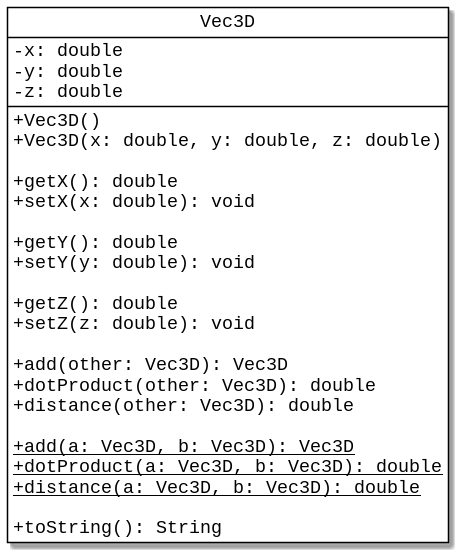
\includegraphics[scale=0.5]{figs/vec3d_a.png}
\caption{UML Diagram with three separate instance variables}
\label{fig.vec3d_a}
\end{center}
\end{figure}

The class has a no-argument constructor (which sets all the coordinates to zero) and a three-argument constructor to set the {\em x}, {\em y}, and {\em z} coordinates explicitly.

These are followed by the getters (accessors) and setters (mutators) for each of the dimensions. 

The class specifies an \java{add}, \java{dotProduct}, and \java{distance} instance methods that find the sum, dot product, and distance of the current vector and an ```other'' vector.

For the convenience of users, the class also specifies \java{static} versions of these methods (the convention in UML diagrams is to underline \java{static} elements) where you specify both vectors you want to manipulate.


But wait---you already have code for doing addition, dot product, and vector distance from Exercise~\ref{ex:vectors}. Because your instance variables are private, you can replace \java{x}, \java{y}, and \java{z} with a three-element array of \java{double} values, as in Figure~\ref{fig.vec3d_b}, and use the code that you wrote in that exercise.

\begin{figure}[!h]
\begin{center}
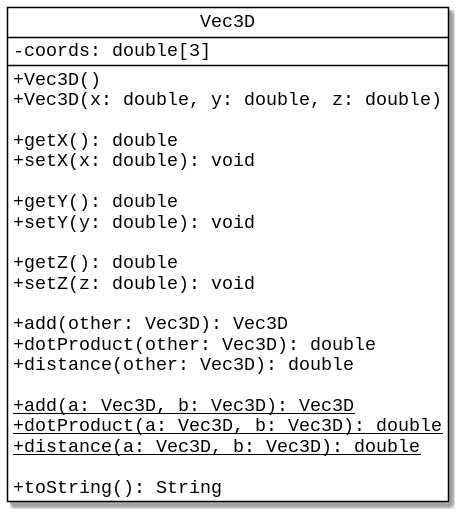
\includegraphics[scale=0.5]{figs/vec3d_b.png}
\caption{UML Diagram with array to hold coordinates}
\label{fig.vec3d_b}
\end{center}
\end{figure}

Notice that the \java{public} methods have not changed; users will never know that the vector is implemented as an array rather than three individual variables.

And that's your job for this exercise: implement the \java{Vec3D} class with a \java{private} array to hold the coordinates. Then, write a \java{main} method that will ask the user to enter two vectors and then display the sum, dot product, and distance between the vectors. To avoid repetitious code, you might want to write a \java{getVector} method that has a prompt and a \java{Scanner} as its parameters. This method will prompt the user for the three vector components and return a \java{Vec3D} object. 

\end{exercise}


\chapter{Arrays of Objects}

\section{Exercises}

\begin{exercise}
Consider this UML diagram for a \java{City} class in Figure~\ref{fig.cityuml}

\begin{figure}[!h]
\begin{center}
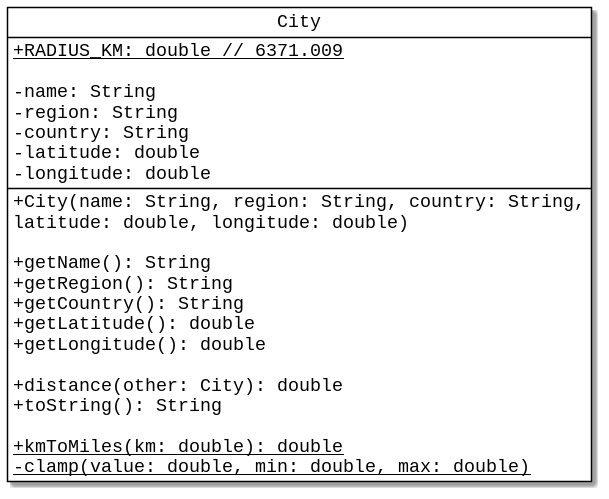
\includegraphics[scale=0.5]{figs/ch12/city.png}
\caption{UML Diagram for a City class}
\label{fig.cityuml}
\end{center}
\end{figure}

The class has private instance variables for the city name, its region (for the US, it's called a state; for Canada, it's a province; for Japan it's a prefecture), and its latitude and longitude measured in degrees.

This is an immutable class. (How would you determine this from the UML diagram?)

\java{RADIUS_KM} is a \java{static} \java{final} constant representing the radius of the earth in kilometers.

The constructor will make sure that the longitude is in the range -180 to 180 and the latitude in the range -90 to 90. The constructor will use the \java{clamp} method to enforce this:

\begin{code}
private static double clamp(double value, double min, double max) {
    double result = value;
    if (value <  min) {
        result = min;
    }
    else if (value > max) {
        result = max;
    }
    return result;
}
\end{code}


Questions: Why do you think this method was declared \java{private} instead of \java{public}? Why is it a \java{static} method instead of an instance method?

The \java{toString} method will display the information about the city; it can display the latitude and longitude as positive and negative numbers, or by using N, S, E, and W as abbreviations for north, south, east, and west. Display them to one decimal point. (Hint: \java{"\\u00b0"} is the degree symbol.) For example:

\begin{stdout}
San Jose, CA, USA: 37.3°, -121.9°
San Jose, CA, USA: 37.3°N, 121.9°W
\end{stdout}


The \java{distance} method will calculate the great circle distance between one \java{City} object and the \java{other} \java{City} object. Here is the formula where $r$ is the radius of earth in kilometers (6371.009), the first city's latitude and longitude are $lat_1$, $lon_1$ and the second city's latitude and longitude are  $lat_2$, $lon_2$:

\begin{equation*}
d = r\cdot cos^{-1}(sin(lat_1)\cdot sin(lat_2) + cos(lat_1)\cdot cos(lat_2)\cdot cos(lon_1 - lon_2))
\end{equation*}

The \java{main} method will set up an array of these \java{City} objects:

\begin{tabular}{|l|l|l|r|r|}
\hline
City & Region & Country & Latitude & Longitude \\ \hline
Antananarivo & Analamanga & MG & -18.93 & 47.52 \\ \hline
Brasilia & Distrito Federal & BR & -15.79 & -47.88 \\ \hline
Mumbai & Maharashtra & IN & 19.08 & 72.88 \\ \hline
Munich & Bavaria & DE & 48.08 & 11.57 \\ \hline
San Jose & California & US & 37.34 & -121.89 \\ \hline
Yokohama & Kanagawa & JP & 35.44 & 139.64 \\ \hline
\end{tabular}

The \java{main} method then prints a list of the cities and the inter-city distances with output as follows. Hint: use \java{"\%8.0f"} to round the distance to an integer:

\begin{stdout}
A: Antananarivo, Analamanga, MG (18.9°S, 47.5°E)
B: Brasilia, Distrito Federal, BR (15.8°S, 47.9°W)
C: Mumbai, Maharashtra, IN (19.1°N, 72.9°E)
D: Munich, Bavaria, DE (48.1°N, 11.6°E)
E: San Jose, California, US (37.3°N, 121.9°W)
F: Yokohama, Kanagawa, JP (35.4°N, 139.6°E)

Inter-city great circle distances in km:
        A       B       C       D       E       F    
A      ----
B      9991    ----
C      5052   13749    ----
D      8264    9214    6325    ----
E     17724    9716   13553    9459    ----
F     11399   17706    6720    9396    8356    ---- 
\end{stdout}

\end{exercise}

\begin{exercise}
Figure~\ref{fig.courseuml} is the UML diagram for a \java{Course} object that represents a college course. The \java{day} attribute gives the day on which the course is taught, with 1 representing Monday and 7 representing Sunday. The \java{startTime} and \java{endTime} are given as integers that represent military time (0000 is midnight and 2359 is 11:59 p.m.)

\begin{figure}[!h]
\begin{center}
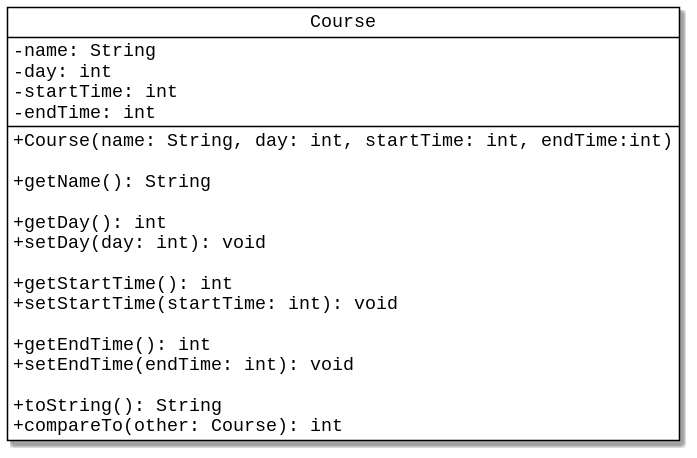
\includegraphics[scale=0.5]{figs/ch12/course.png}
\caption{UML Diagram for a Course object}
\label{fig.courseuml}
\end{center}
\end{figure}

When you write the constructor and the setters, make sure that the day of week is always in the range 1-7 and that the times are in the range 0000-2359. Make sure you handle a time like 2079 in some reasonable fashion---you decide what ``reasonable'' means here, and {\bf use comments to document it}. You may want to rewrite the \java{clamp} method from the preceding exericse to use integers as its parameters and return value. Then you can use it when writing a new \java{clampTime} method to enforce these conditions.

Note: a constructor can call an instance method; that is, the constructor for \java{Course} can call the \java{setDay}, \java{setStartTime}, and \java{setEndTime} methods. This will eliminate a lot of duplicated code.

The \java{compareTo} method uses the following criteria when doing a comparison: First, compare the \java{day} attributes. If they aren't equal, then return 1 or $-1$ (depending on which one is less or greater). If the \java{day} fields are equal, compare the \java{startTime} attributes and return 1, 0, or $-1$ depending on their relationship.

The \java{toString} method will display the course's attributes. Again, you decide what you want it to look like.

In the \java{main} method, create an array of the following courses, in this order. Note that ECON 010A has an invalid time so that you can test to see what your code does:

\begin{tabular}{|l|l|l|l|}
\hline
Name & Day & Start Time & End Time \\ \hline
ACCTG 001A & 1 & 1515 & 1645 \\ \hline
BIO 020 & 3 & 1235 & 1540 \\ \hline
COMSC 075 & 2 & 0915 & 1125 \\ \hline
ECON 010A & 4 & 1515 & 1679 \\ \hline
MATH 063 & 1 & 0915 & 1035 \\ \hline
PSYCH 018 & 3 & 1615 & 1750 \\ \hline
THEAT 034 & 1 & 1215 & 1335\\ \hline
\end{tabular}

Then, iterate through the array to find the courses with the earliest and latest start times according to the \java{compareTo} method.

\begin{minipage}[t]{0.8\textwidth}

\noindent\rule{\textwidth}{1pt}

{\bf NOTE:} You cannot do this in Java:
\begin{code}
int startTime = 0915;
\end{code}

The reason is that a leading zero indicates to Java that your number is {\em octal} (base 8), and there is no digit 9 in that number base. Instead, leave off the leading zero:

\begin{code}
int startTime = 915;
\end{code}

You do not have to worry about this when doing user input; the \java{nextInt} and \java{Integer.parseInt} methods use decimal (base 10) by default, so when a person enters the string \java{0915} it will be converted to integer without an error.

\noindent\rule{\textwidth}{1pt}

\end{minipage}

Sample output:

\begin{stdout}
Earliest course: MATH 063: M (0915-1035)
Latest course: ECON 010A: Th (1515-1659)
\end{stdout}

\end{exercise}


\chapter{Objects of Arrays}




\chapter{Extending Classes}

\section{Composition and Inheritance}

Two important concepts in object-oriented programming are {\em composition} and {\em inheritance}. In {\em Think Java, 2nd Edition}, you have seen composition in Chapter 13 and inheritance in Chapter 14, but mostly by example. We're going to go into more detail on both of these concepts here.

\section{Composition}
\index{composition}
\index{aggregating class}
\index{aggregated class}
\index{class!aggregating}
\index{class!aggregated}

Composition happens when an object is made up of other objects. We saw this in Chapter 13, where a \java{Deck} was made up of an array of \java{Card} objects:

\begin{code}
public class Deck {
    private Card[] cards; 
    ...
}
\end{code}

Composition is also known as a {\em Has-A} relationship.  (A \java{Deck} {\em has an} array of \java{Card}s).  Put formally, the \java{Deck} is the {\em aggregating class}, and the \java{Card} class is is the {\em aggregated class}.

When we draw a UML diagram involving composition, as in Figure~\ref{fig.aggregation}, we use an arrow with a diamond head to indicate aggregation, and we can also add notation here that shows that one \java{Deck} contains many \java{Card} objects.

\begin{figure}[!h]
\begin{center}
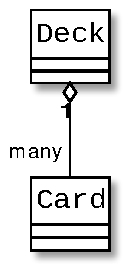
\includegraphics[scale=0.75]{figs/ch14/aggregation.pdf}
\caption{UML Diagram Showing Aggregation - a Deck has Card(s)}
\label{fig.aggregation}
\end{center}
\end{figure}

Let's use composition to build a Java simulation of a toaster. What things is a toaster built from?

\begin{itemize}
\item A chassis with a number of slots
\item A lever to push bread down or pop it out
\item A power supply to turn the toaster on and off
\item A dial to control the darkness (1=light, 10=dark)
\end{itemize}

The first two of these are built by the toaster company. But the company that makes toasters doesn't build the power supply or the dial (which has circuitry to control the current built into it). Instead, those are parts they order from some other companies and use those to put into the chassis.

That means that our \java{Toaster} {\em has-a} \java{PowerSupply} object and {\em has-a} \java{Dial} object. Figure~\ref{fig.toasterComposition} shows the UML diagram. You can see the full code in the file {\em ch14/ToasterTest.java} in the repository.

\begin{figure}[!h]
\begin{center}
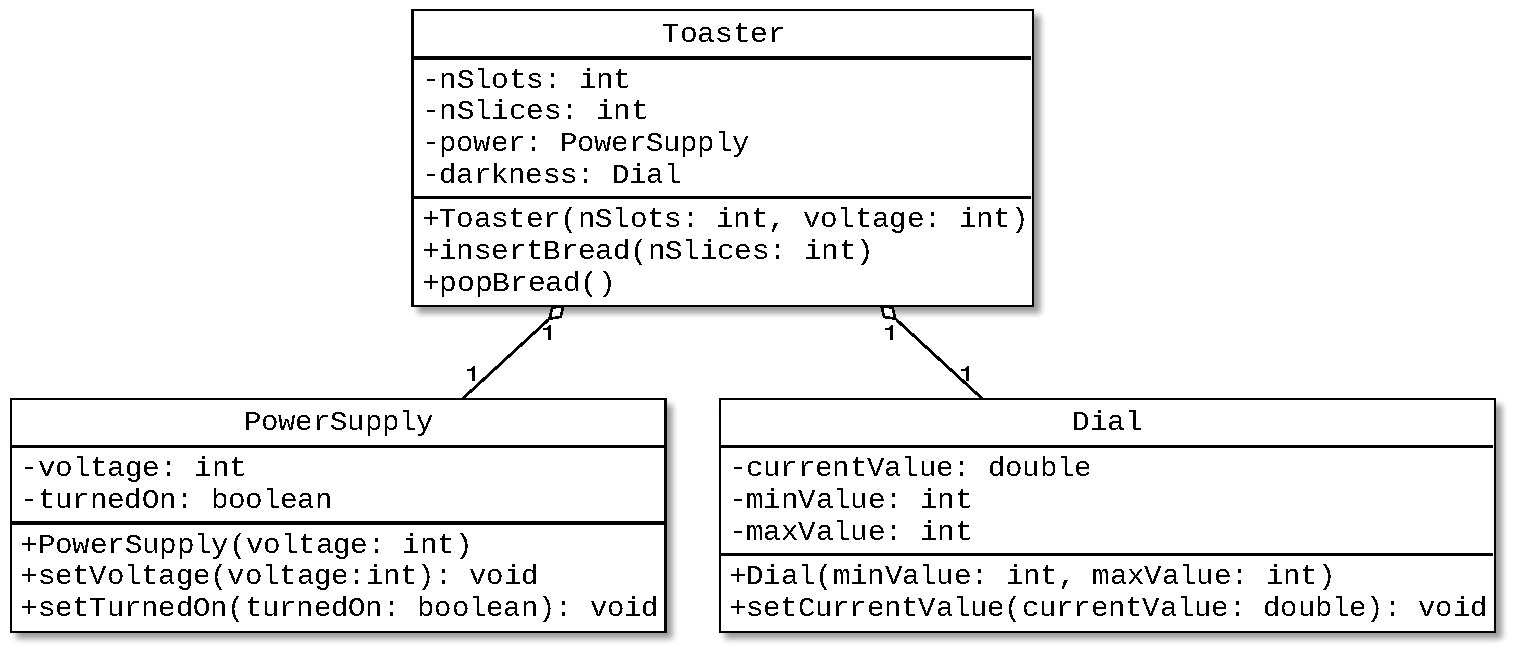
\includegraphics[scale=0.5]{figs/ch14/toaster.pdf}
\caption{UML Diagram Showing a Toaster composed of a PowerSupply and Dial}
\label{fig.toasterComposition}
\end{center}
\end{figure}

Before we see how composition affects the way we construct and manipulate objects, let's give a few more instances of composition ({\em has-a}) relationships. Using composition reflects the way objects are built out of other objects (parts). Each of the sub-parts has its own attributes and things that it can do (its ``methods''). Notice that we sometimes need multiple sub-parts when constructing the larger object.

\begin{itemize}
\item A printer has a power supply, printer drum, and toner cartridge.
\item A bicycle has a gear assembly, handbrakes (2), and tires (2).
\item A refrigerator has a power supply, an icemaker, and a compressor.
\item A window in a word processor has a text area, a ribbon (icons for manipulating text), and two scroll bars (horizontal and vertical).
\end{itemize}

Back to the toaster. Here are constructors for the \java{PowerSupply} and \java{Dial} classes:

\begin{code}
public PowerSupply(int voltage) {
    this.voltage = voltage;
    // new power supplies are always shipped in the "off" position
    this.turnedOn = false;
}

public Dial(int minValue, int maxValue) {
    this.minValue = minValue;
    this.maxValue = maxValue;
    // new dials are always set to lowest value
    this.currValue = minValue;
}
\end{code}

Now, look at how the \java{Toaster} class starts, with line numbers for reference:

\begin{code}
 1 class Toaster {
 2     private int nSlots;
 3     private int nSlices;
 4     private PowerSupply power;
 5     private Dial darkness;
 6  
 7     public Toaster(int nSlots, int voltage) {
 8         this.nSlots = nSlots;
 9         this.nSlices = 0;
10         this.power = new PowerSupply(voltage);
11         this.darkness = new Dial(1, 10);
12     }
13     // ...
14 }
\end{code}

The constructor in line 7 has two parameters: the number of slots in the toaster and what voltage it should have. The number of slots and number of slices of bread currently in the toaster are attributes belonging to the \java{Toaster} class, and those get set directly.

The power supply is an object, which is why line 10 has to call the \java{PowerSupply} constructor to build a power supply with the desired voltage. Think of this as the toaster company calling up the power supply company and telling them “send me a 110-volt power supply” and putting that power supply into the finished toaster.

Similarly, line 11 has to call the \java{Dial} constructor to build a dial with a range of 1-10.

When we start using a newly created \java{Toaster} object, we have to remember that it is composed of other objects:

\begin{code}
 1 public class ToasterTest {
 2     public static void main(String[] args) {
 3         Toaster northAmTwo = new Toaster(2, 110);
 4         Toaster euroFour = new Toaster(4, 220);
 5        
 6         northAmTwo.getPower().setTurnedOn(true);
 7         northAmTwo.getDarkness().setCurrentValue(4);
 8         northAmTwo.insertBread(1);
 9         
10         System.out.println(northAmTwo);
11         System.out.println(euroFour);
12     }
13 }
\end{code}

Line 3 creates a two-slot, 110-volt toaster for North America; line 4 creates a four-slot, 220 volt toaster for Europe.
Things get interesting on line 6 when we turn on the North America toaster. Read from right to left, line 6 says “call the \java{setTurnedOn} method belonging to the power supply belonging to the \java{northAmTwo} toaster.

We can {\em not} say this:

\begin{code}
northAmTwo.setTurnedOn(true);
\end{code}

because the \java{setTurnedOn} method belongs to the \java{PowerSupply} class, not the \java{Toaster} class.  (We need to use \java{getPower} because the \java{power} attribute in the \java{Toaster} class is \java{private}.)

To summarize this discussion of composition:

\begin{itemize}
\item Use composition when you have objects that are built up from other objects.
\item When you need to access an attribute or a method of a sub-part of an object, use notation like \java{object.getSubPart().method()} or \java{object.getSubPart().getAttribute()}. (This presumes that the sub-parts and their attributes are \java{private})
\end{itemize}

\section{Exercises}

\begin{exercise}
In this exercise, we will explore {\em has-a} and {\em is-a} relationships.


An {\em Is\-A} relationship is known as {\em inheritance}. For example, a \java{Hand} class (subclass) is also a \java{CardCollection} class (superclass). In Java, we use \java{extends} to indicate inheritance:

\begin{code}
public class Hand extends CardCollection {
   ...
}
\end{code}

Figure~\ref{fig.simpleInheritance} shows the UML for inheritance, using an open arrowhead:

\begin{figure}[!h]
\begin{center}
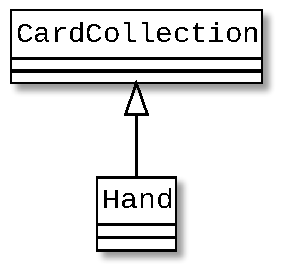
\includegraphics[scale=0.75]{figs/ch14/inheritance.pdf}
\caption{UML Diagram Showing Inheritance - a Hand is a CardCollection}
\label{fig.simpleInheritance}
\end{center}
\end{figure}

First, state whether the relationship of the following classes is composition or inheritance, and draw the UML diagram showing that relationship.

\begin{itemize}
    \item \java{Address} and \java{Student}
    \item \java{Car} and \java{Vehicle}
    \item \java{Account} and \java{SavingsAccount}
    \item \java{State}, \java{Capital}, and \java{Country}
    \item \java{Instructor}, \java{Course}, and \java{Textbook}
    \item \java{Dog}, \java{Cat}, and \java{Animal}
    \item \java{Rectangle}, \java{Circle}, \java{Square}, and \java{Shape}
\end{itemize}


For classes that exhibit the inheritance relationship, could you name a few data fields/attributes for the superclass? Could you name a few for the subclass only?

For example, \java{Teacher} (subclass) is also a \java{Person} (superclass). 
Data fields for \java{Person} are: name, age, address, etc.
Data fields for \java{Teacher} are: school, hire date etc.

\end{exercise}

\begin{exercise}
Design a class named \java{Person} with two subclasses: \java{Employee} and \java{Customer}. The attributes for these classes are described in italics. A \java{Person} has a {\em name}, {\em address}, {\em phone number}, and  {\em email address}.

An \java{Employee} has an {\em employee number}, {\em hire date}, and {\em salary}.

The \java{Employee} class, in turn, has three subclasses: \java{Programmer}, \java{Tester}, and \java{Manager}. 
\begin{itemize}
\item A \java{Programmer} and a \java{Tester} have a {\em cubicle number}. Both will receive a {\em fixed bonus} at the end of the year.
\item A \java{Manager} has an {\em office number} and has a variable bonus based on the performance of their team. This means that a \java{Manager} should have attributes for the {\em target bonus amount} and the {\em performance percentage}.
\end{itemize}

Finally, the \java{Customer} should have a {\em customer number} and {\em company} they work for.

Draw the UML diagram showing the relationship of these classes, then code all these classes showing the data fields and attributes. Make meaningful names for the attributes and give them an appropriate data type. (You do not need to create constructors or other methods for the classes.)
\end{exercise}

\begin{exercise}
The XYZZY Corporation wants to retain their most loyal customers. They launch a customer retention program and offer discount to customers who have been purchasing from the company for at least one year.

Write a subclass \java{PrefCust} that extends the \java{Customer} class from the preceding exercise. The \java{PrefCust} class should have two data fields: {\em purchase amount} and {\em customer history} (number of years they have been a customer). These are both private variables.

Customers get a discount percentage based on their history and purchase amount. There are three levels of Preferred Customers: bronze, silver and gold.

\begin{itemize}
\item Bronze: history $\geq$ 1 year and average purchase amount $\geq$ \$5000 per year.  5%% off
\item Silver:  history $\geq$ 2 years and average purchase amount $\geq$ \$10000 per year. 7.5%% off
\item Gold:  history $\geq$ 3 years and average purchase amount $\geq$ \$15000 per year. 10%% off
\end{itemize}

The discount percentage is a {\em derived attribute}---it is never set directly, but instead is computed based on other attributes.

Write the \java{PrefCust} class with all its data fields. Please write all the getter and setter methods.  Write a method named \java{getDiscountPercent} that uses the purchase amount and customer history to return the discount percent (as a percentage).
\end{exercise}

%=========================================

\begin{exercise}

In this exercise, you will implement an \java{Account} class which represents a bank checking account. You will then create two classes that inherit from \java{Account}: \java{SavingsAccount} and \java{CreditCardAccount}.

You will then use composition to create a \java{Customer} class which includes instances of each of these account classes.

Finally, you will write a program with a \java{main} method that tests these classes.

{\bf Part 1}: Create a class named \java{Account}, which has the following private properties:

\begin{itemize}
    \item \java{number: long}
    \item \java{balance: double}
\end{itemize}

\begin{enumerate}
\item Create a two-parameter constructor that takes an account number and balance. Make sure that the balance is always greater than zero ({\em Hint}: \java{Math.abs})

\item Implement getters and setters: \java{getNumber()}, \java{getBalance()}, \java{setBalance(double newBalance)}. There is no \java{setNumber} method---once an account is created, its account number cannot change.

\item Implement these methods: \java{void deposit(double amount)} and \java{void withdraw(double amount)}. For both these methods, if the amount is less than zero, the account balance remains untouched. For the \java{withdraw} method, if the amount is greater than the balance, it remains untouched. {\em These methods do not print anything.}

\item Implement a \java{toString} method that returns a string with the account number and balance, properly labeled.
\end{enumerate}

{\bf Part 2}: Next, implement the \java{SavingsAccount} class. It inherits from \java{Account} and adds a private \java{apr} property, which is the annual percentage rate (APR) for interest.

\begin{enumerate}
\item Write a three-argument constructor that takes an account number, balance, and interest rate as a decimal (thus, a 3.5\% interest rate is given as 0.035). Make sure that the interest rate is never less than zero.

\item add a getter and setter: \java{getApr()} and \java{setApr(double apr)}. The setter must ensure that the APR is never less than zero.

\item Write a \java{calculateInterest} instance method that returns the annual interest, calculated as the current balance times the annual interest rate.

\item Modify \java{toString} to include the interest rate. IMPORTANT: The value returned by the \java{toString} method must {\bf {\em not}} include the calculated annual interest.
\end{enumerate}

{\bf Part 3}: Next, implement the \java{CreditCardAccount} class, which inherits from \java{Account} and adds these \java{private} properties:

\begin{itemize}
\item \java{apr}, a \java{double} representing the annual interest rate charged on the balance.
\item \java{creditLimit}, a \java{double} which gives the credit limit for the card.
\end{itemize}

Then, implement:
\begin{enumerate}
\item A four-argument constructor that takes an account number, balance, interest rate as a decimal (thus, a 3.5\% interest rate is given as 0.035), and credit limit. Make sure that neither the interest rate nor credit limit can be negative.

\item Write getters and setters for the \java{apr} and \java{creditLimit}. The apr setter should leave the APR untouched if given a negative value. The \java{creditLimit} setter should leave the credit limit untouched if given a negative value.

\item Modify \java{toString} to include the interest rate and credit limit. IMPORTANT: the value returned by the \java{toString} method must {\bf {\em not}} include the monthly payment.

\item Override the \java{withdraw} method so that you can have a negative balance. If a withdrawal would push you over the credit limit, leave the balance untouched. Examples:

\begin{itemize}
\item If your balance is \$300 with a credit limit of \$700, you can withdraw \$900 (leaving a balance of \$-600).
\item If your balance is \$-300 with a credit limit of \$700, you can withdraw \$350 (leaving a balance of \$-650).
\item If your balance is \$-300 with a credit limit of \$700, you can not withdraw \$500, because that would then owe \$800, which is more than your \$700 limit.
\end{itemize}

In short, the maximum amount you can withdraw is your current balance plus the credit limit.

%\item Implement a \java{calculatePayment} method that works as follows: If the balance is positive, the minimum amount you have to pay on your card per month is zero. Otherwise, your monthly payment is the minimum of 20 and $(apr/12) \cdot (−balance)$

\end{enumerate}

{\bf Part 4}: Now, write a \java{Customer} class that will use composition to include the preceding classes.

\begin{enumerate}
\item The \java{Customer} class has the following private attributes:

\begin{itemize}
\item \java{name: String}
\item \java{acct: Account}
\item \java{savings: SavingsAccount}
\item \java{credit: CreditAccount}
\end{itemize}

\item Implement a four-argument constructor for this class.

\item Write getters and setters for all the fields.
\end{enumerate}

Figure~\ref{fig.inheritance1} shows the details of the \java{Account} class and its subclasses. Figure~\ref{fig.inheritance2} shows the relationships of all the classes in this exercise.

\begin{figure}[!ht]
\begin{center}
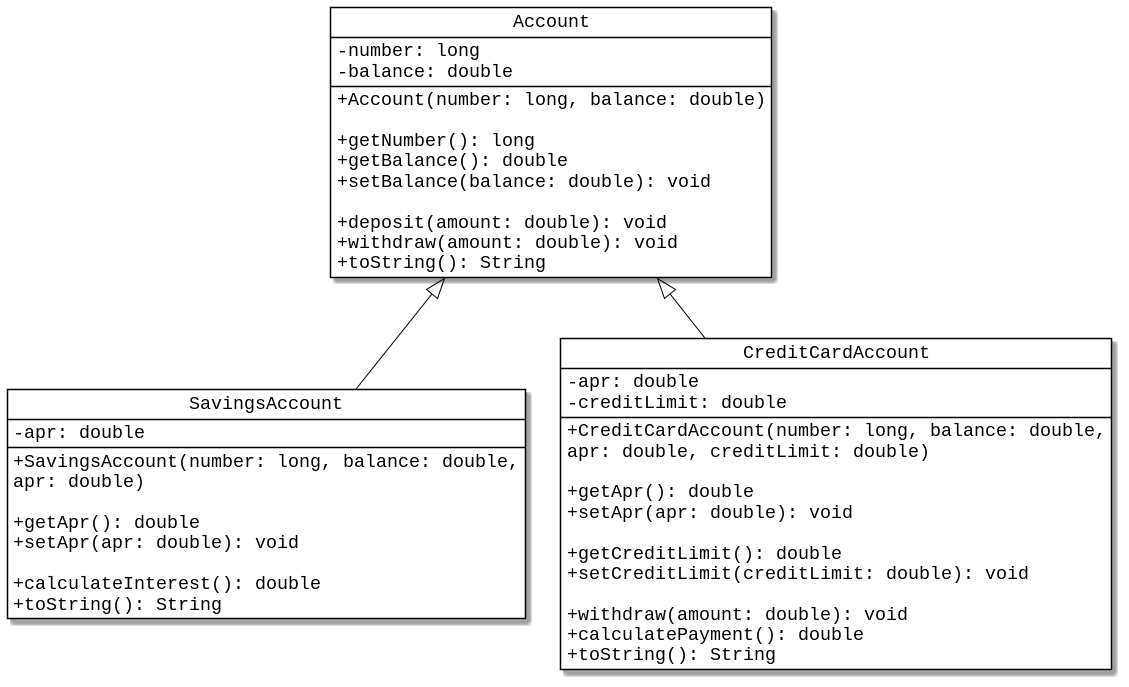
\includegraphics[scale=0.4]{figs/ch14/account_inheritance.png}
\caption{\java{Account}, \java{SavingsAccount}, and \java{CreditCardAccount} classes}
\label{fig.inheritance1}
\end{center}
\end{figure}

\begin{figure}[!ht]
\begin{center}
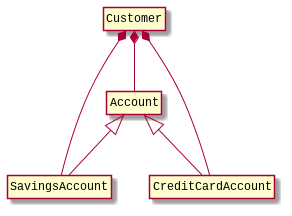
\includegraphics[scale=0.7]{figs/ch14/account_classes.png}
\caption{Composition and Inheritance Among All Classes}
\label{fig.inheritance2}
\end{center}
\end{figure}

{\bf Part 5}: Finally, write a program named {\em TestCustomer.java} that creates a \java{Customer} named ``Joe Doakes'' with this data:

\begin{itemize}
\item Regular account number 1037825 with a balance of \$3,723.00
\item Savings account number 9016632 with a balance of \$4,810.25 and an annual interest rate of 2.05\%
\item Checking account number 85332162 with a balance of -\$2500.00, an interest rate of 7.125\%, and a credit limit of \$3000.00.
\end{itemize}

Then, do the following transactions:

\begin{itemize}
\item Deposit \$257.18 into the regular account, then withdraw \$587.23.
\item Deposit \$2,466.12 into the savings account, then withdraw \$8,000.00.
\item Withdraw \$480.00 from the credit card account.
\item Display the status of the regular account (number and balance).
\item Display the status of the savings account (number, balance, and annual interest amount).
\item Display the status of the credit card account (number, balance, interest rate, and monthly payment due).
\end{itemize}


\end{exercise}


\chapter{Arrays of Arrays}

\section{Initializing Two-Dimensional Arrays}
You already know that you can initialize a one-dimensional array by putting the values in braces:

\begin{code}
int[] ages = {35, 27, 45, 58};
\end{code}

Because two-dimensional arrays are stored in Java as an array of arrays, as shown in Figure~\ref{fig:2D-array}, you can initialize them in a simliar manner.

\begin{figure}[!ht]
\begin{center}
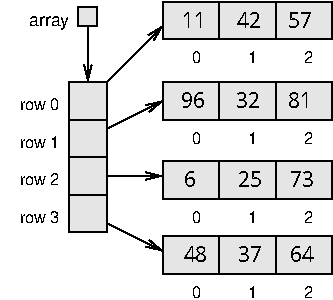
\includegraphics{figs/ch15/2D-array.pdf}
\caption{Storing rows and columns with a 2D array.}
\label{fig:2D-array} 
\end{center}
\end{figure}

\begin{code}
int[ ][ ] array = {
    {11, 42, 57},
    {96, 32, 81},
    { 6, 25, 73},
    {48, 37, 64}
};
\end{code}

However, there are times that we need to be able to read two-dimensional arrays from a user. It would be useful to have a small library of code that would allow us to read and print two-dimensional arrays so that we would not have to copy and paste the code into every program that needs it. That is the subject of the next section and the second exercise.

\section{Programs in Multiple Files}
Up to this point, all of our Java programs have been written in one file. We have used \java{import} to bring in classes and methods from other files.  Now it’s time to learn how to do this ourselves. There are many ways to structure a program so that it can be divided into separate files that are brought together at run time; the method we're using here is the simplest.

As an example, let's say we would like to have some methods that are generally useful for doing statistics with arrays of \java{double} values. We'll put them into a \java{public} class of their own. The following code gives the outline; you can download the entire file from the code repository at \url{https://github.com/jdeisenberg/ThinkJava2ExCode}

\begin{code}
public class ArrayStats {

    public static double mean(double[ ] data) {
        // calculation code goes here
        return result;
    }
    
    public static double stdv(double[ ] data) {
        // code goes here
        return result;
    }
}
\end{code}

You can now use these methods from another program, say, \java{TestStats.java} by putting the \java{ArrayStats.java} file in the same directory as the \java{TestStats.java} file.  If you do this, you don't need to do an \java{import}:

\begin{code}
public class TestStats {

    public static void main(String[ ] args) {
        double [ ] values = {10.0, 47.0, 6.6, 505.0217, 11.0};
        double avg = ArrayStats.mean(values);
        double stdDev = ArrayStats.stdv(values);
        System.out.printf("Average: %.3f\n", avg);
        System.out.printf("Standard Deviation: %.3f\n", stdDev);
    }
}
\end{code}

More complex ways of dividing a Java program into separate files involves the concepts of \java{package} and \java{module}. You can see documentation about this at \url{https://docs.oracle.com/javase/specs/jls/se9/html/jls-7.html}. 

\section{Exercises}

\begin{exercise}
Create a two-dimensional array of \java{int} that represents the following table of sales (in thousands of units), measured quarterly for three years. The first row and the leftmost column won't be part of your table; they are here to label the items properly so you can understand how the table is structured.

\begin{tabular}{|l|l|l|l|l|}
\hline
Year & Q1 & Q2 & Q3 & Q4 \\ \hline
1     & 27 & 24 & 29 & 28 \\ \hline
2     & 36 & 38 & 34 & 33 \\ \hline
3     & 34 & 39 & 37 & 36 \\ \hline
\end{tabular}

Then, have your program calculate and print:

\begin{itemize}
\item The total sales for each of the three years
\item The total sales for each quarter (across the three years)
\item The grand total of sales
\end{itemize}
\end{exercise}

\begin{exercise}
In this exercise, you'll write methods for doing input and output of a two-dimensional array. Put these methods into a file named \java{IO2D.java} (standing for Input/Output 2D). You will use these methods in the subsequent exercises.

{\bf Input}: Write a \java{public static double[ ][ ]} method named \java{getDoubleArray2D} with four parameters:

\begin{itemize}
\item A \java{Scanner} object
\item The prompt for the description of the array to enter (\java{String})
\item The number of rows (\java{int})
\item The number of columns (\java{int})
\end{itemize}

The method returns a two-dimensional array of \java{double}. For example, you might call it as:

\begin{code}
double [ ][ ] temps = getIntArray2D(input,
  "Enter temperature data one row at a time", 7, 3);
\end{code}

{\bf Output}: Write a \java{public static void} method named \java{printDoubleArray2D}, with two parameters:
\begin{itemize}
\item A formatting \java{String} like you would use in \java{System.out.printf} or \java{String.format}.
\item The array to be printed
\end{itemize}

This method will print out the arrays, using the given format for each element in the array. You might call it
like this:

\begin{code}
printDoubleArray2d(temps, "%.1f");
\end{code}

Then, in a class named \java{TestInputOutput}, write a \java{main} method that creates a 3 row, 4 column array of \java{double} and calls \java{getDoubleArray2D} and \java{printDoubleArray2D} to read an array and print it out. 

Here is sample output from this code:

\begin{code}
double[ ][ ] values = IO2D.getArray2d(input,
    "Enter three rows of data, one row at a time.", 3, 4);
System.out.println();
System.out.println("Here is your data:");
IO2D.printArray2d("%7.1f", values);
\end{code}

\begin{stdout}
Enter three rows of data, one row at a time.
Enter 4 items for row 1: 3.4 7.8 2.93 -12.1
Enter 4 items for row 2: 14.4 8.75 3.45 18.2225
Enter 4 items for row 3: 31.2 -56.4 19.21 47.66

Here is your data:
    3.4     7.8     2.9   -12.1 
   14.4     8.8     3.5    18.2 
   31.2   -56.4    19.2    47.7 
\end{stdout}

\end{exercise}

\begin{exercise}
In this exercise and the following exercises, you will develop methods that do mathematics with two-dimensional arrays, also called {\em matrices}.  Create a file named \java{MatrixMath.java}, which will have a \java{public class MatrixMath}.

First, write a method that adds two matrices. You do this by adding the corresponding entries of the two matrices:

\begin{equation*}
\begin{pmatrix}
1 & 2 & 3 \\
4 & 5 & 6 \\
7 & 8 & 9
\end{pmatrix}
+
\begin{pmatrix}
10 & 11 & 12 \\
13 & 14 & 15 \\
16 & 17 & 18
\end{pmatrix}
\rightarrow
\begin{pmatrix}
11 & 13 & 15 \\
17 & 19 & 21 \\
23 & 25 & 27
\end{pmatrix}
\end{equation*}

Here is the signature of the method:

\begin{code}
public static double[][] add(double[][] arr1, double[][] arr2)
\end{code}

The two arrays must have the same number of rows and columns. Write a method named \java{isAddCompatible} that will do that test for the users of your code. The method returns \java{true} if the arrays can be added, \java{false} otherwise. Its signature is:

\begin{code}
public static boolean isAddCompatible(double[][] arr1, double[][] arr2)
\end{code}

To test these methods, write a separate file with a \java{main} method that:

\begin{itemize}
\item Asks the user for the dimensions of one array and reads it in.
\item Asks the user for the dimensions of another array and reads it in.
\item If the arrays are compatible, add them and print the resulting array. If not, print an appropriate error message.
\end{itemize}

\end{exercise}

\begin{exercise}
Add a method to the \java{MatrixMath} class:

\begin{code}
public static double[][] scale(double[][] arr, double factor)
\end{code}

This method returns a new array the same size as the input array, with each element in the array multiplied by the given factor. Write a test program in a separate file that asks the user for the dimensions of an array, reads it in, asks for a scaling factor, reads that in, and scales the elements by the given factor and prints the result.
\end{exercise}

\begin{exercise}
Adding matrices is fairly straightforward. Multiplying them is anything but! In this exercise, you will write a method to multiply two matrices. The header of the method is:

\begin{code}
public static double[][] multiply(double[][] a, double [][] b)
\end{code}

To multiply a matrix $a$ by matrix $b$, the number of columns in $a$ must be the same as the number of rows in $b$, and the two matrices must have elements of the same or compatible types. Let $c$ be the result of the multiplication. Assume that $a$ has $n$ columns. Each element $c_{ij}$ is $a_{i1} \times b_{1j} + a_{i2} \times b_{2j} + ... + a_{in} \times b_{nj}$. For example,

\begin{align*}
\begin{pmatrix}
1 & 2 & 3 \\
4 & 5 & 6 \\
\end{pmatrix}
\times
\begin{pmatrix}
7 & 10 \\
8 & 11 \\
9 & 12
\end{pmatrix}
=
\end{align*}
%
% PDFLatex doesn't seem to like splitting into lines
% if I add a blank line; it gives errors. Hence
% I have to start a new equation.
%
\begin{align*}
\begin{pmatrix}
1\cdot 7+2\cdot 8+3\cdot 9 & 4\cdot 7+5\cdot 8+6\cdot 9\\
1\cdot 10+2\cdot 11+3\cdot 12 &  4\cdot 10+5\cdot 11+6\cdot 12\\
\end{pmatrix}
=
\begin{pmatrix}
50 & 68\\
122 & 167
\end{pmatrix}
\end{align*}

Implement a method with this header:

\begin{code}
public static boolean isMultiplyCompatible(double [][] arr1,
    double [][] arr2)
\end{code}

This will return \java{true} if the number of columns in \java{arr1} is equal to the number of rows in \java{arr2}, \java{false} otherwise.

Your \java{main} method will prompt the user for the number of rows and columns for the first matrix, then its contents. It will then prompt the user for the number of rows and columns for the second matrix, then its contents. It will then determine if the matrices are compatible by calling \java{isMultiplyCompatible}. If the matrices are compatible, the program will call the \java{multiply} method and print the returned matrix. If not, it will print an appropriate error message.

Here is an example of a run of the program:

\begin{stdout}
Matrix A
Enter number of rows: 2
Enter number of columns: 3
Enter contents by rows: 1 2 3 4 5 6
Matrix B
Enter number of rows: 3
Enter number of columns: 2
Enter contents by rows: 7 10 8 11 9 12

Matrix C is
50.0 68.0 
122.0 167.0
\end{stdout}

\end{exercise}


\chapter{Reusing Classes}

\section{Exercises}


\chapter{Advanced Topics}

\section{Exercises}




\chapter{Exceptions and Files}

\section{Exceptions}

Consider this program:

\begin{code}
import java.util.Scanner;

public class ErrorProne {

    public static void main(String[] args) {
        int[] data = {10, 66, 47, 11};
        
        Scanner input = new Scanner(System.in);
        
        System.out.print("Enter index 0-3: ");
        int index = input.nextInt();
        
        System.out.print("Enter number to divide by: ");
        int divisor = input.nextInt();
        
        int result = data[index] / divisor;
        System.out.printf("quotient of %d and %d is %d\n",
            data[index], divisor, result);
    }
}
\end{code}

If you enter a non-number the program crashes:

\begin{stdout}
Enter index 0-3: two
Exception in thread "main" java.util.InputMismatchException
	at java.base/java.util.Scanner.throwFor(Scanner.java:939)
	at java.base/java.util.Scanner.next(Scanner.java:1594)
	at java.base/java.util.Scanner.nextInt(Scanner.java:2258)
	at java.base/java.util.Scanner.nextInt(Scanner.java:2212)
	at ErrorProne.main(ErrorProne.java:11)
\end{stdout}
\index{stack trace}
The lines beginning with \texttt{at} are a {\em stack trace}. They show the chain of method calls in reverse chronological order with the file name and line number. You'll want to look for the one that is in your program. In this case, the error was in \texttt{ErrorProne.java:11}, where the \texttt{11} is the line number in the source file with the \java{nextInt} call.

If you enter an index outside the array bounds, the program crashes (the output has been reformatted to fit on the line length of this page):

\begin{stdout}
Enter index 0-3: 5
Enter number to divide by: 0
Exception in thread "main"
  java.lang.ArrayIndexOutOfBoundsException:
  Index 5 out of bounds for length 4
	at ErrorProne.main(ErrorProne.java:21)

\end{stdout}

And if you enter a zero as the divisor, you get yet another error:

\begin{stdout}
Enter index 0-3: 2
Enter number to divide by: 0
Exception in thread "main"
  java.lang.ArithmeticException: / by zero
    at ErrorProne.main(ErrorProne.java:21)
\end{stdout}

All of these errors are called {\em exceptions}---exceptional conditions after which the program cannot continue to run. In Java, we say that the program {\em throws} an exception when it fails.

You already know how to handle these problems before they crash your program: you can use an \java{if} statement with \java{Scanner}'s \java{hasNextInt} method to make sure that the user enters an integer. You can use \java{if} statements to check that the index number is between 0 and the array's length, and that the divisor is non-zero.

\index{\java{try}}
\index{\java{catch}}
In addition to using an \java{if} statement to avoid errors, Java has another general mechanism for catching exceptions before they stop your program:  \java{try} and \java{catch}.

Let's enclose the code that could have an error in a \java{try} block:

\begin{code}
try {
    System.out.print("Enter index 0-3: ");
    int index = input.nextInt();
    
    System.out.print("Enter number to divide by: ");
    int divisor = input.nextInt();
    
    int result = data[index] / divisor;
    System.out.printf("quotient of %d and %d is %d\n",
        data[index], divisor, result);
}
\end{code}

The \java{try} block is followed by a \java{catch} block that specifies the exception we want to handle
and how to handle it.  Let's start with the division by zero, which generated a \java{java.lang.ArithmeticException}:

\begin{code}
catch (ArithmeticException ex) {
    System.out.println("Number to divide by cannot be zero.");
}
\end{code}

If you recompile and run the program and enter \texttt{2} and \texttt{0} as your numbers, you'll get the error message in the \java{catch} block. Notice that the \java{printf} statement after the division doesn't occur---when an exception is thrown, execution imediately jumps to the \java{catch}.

If you enter \texttt{five} or \texttt{5} for the first input, you'll still get the \java{NumberFormatException} or \java{ArrayIndexOutOfBoundsException}.
 
You may follow a \java{try} block with as many \java{catch} blocks as you want. Let's add two more \java{catch} blocks to handle these other two errors:

\begin{code}
catch (NumberFormatException ex) {
    System.out.println("You must enter digits for numbers.");
}
catch (ArrayIndexOutOfBoundsException ex) {
    System.out.printf("Index must be in range 0-%d\n", data.length);
}
\end{code}

The variable in parentheses after \java{catch} is local to the \java{catch} block. This means you can use the same variable name in all the \java{catch} blocks, and, by convention, most programmers name it \java{ex}. (We will put it to use later in the chapter.)

When an exception occurs, Java goes through the \java{catch} blocks in the order that they appear in your program and finds the first one that applies. In the preceding example, we could have put the \java{catch} blocks in any order. However, the order does become important once we examine the hierarchy of exceptions.

\section{The Hierarchy of Exceptions}
\index{exceptions!hierarchy}
All exceptions descend from the \java{Exception} class\footnotemark. This list shows many of the most common exceptions you will encounter when learning Java; each category contains many other classes:

\footnotetext{\java{Exception} is a child of the \java{Throwable} class. Another child of \java{Throwable} is \java{Error}, which is used for serious, system-level problems. You will very rarely encounter one of these.}

\begin{itemize}
    \item \java{Exception}
        \begin {itemize}
            \item \java{IOException}
                \begin{itemize}
                    \item \java{FileNotFoundException}
                \end{itemize}
            \item \java{RunTimeException}
            \begin {itemize}
                \item \java{ArithmeticException}
                \item \java{IllegalArgumentException}
                    \begin{itemize}
                        \item \java{IllegalFormatException}
                        \item \java{InvalidParameterException}
                        \item \java{NumberFormatException}
                    \end{itemize}
                \item \java{IndexOutOfBoundsException}
                    \begin{itemize}
                        \item \java{ArrayIndexOutOfBoundsException}
                        \item \java{StringIndexOutOfBoundsException}
                    \end{itemize}
                \item \java{NullPointerException}
              \end{itemize}
    \end{itemize}
\end{itemize}

If you put a \java{catch} for a parent class {\em before} a \java{catch} for a child class, the parent class will catch the error.
Thus, in this code fragment:

\begin{code}
try {
    int n = 12 / 0;
}
catch (Exception ex) {
    System.out.println("Something unexpected occurred.");
}
catch (ArithmeticException ex) {
    System.out.println("You can't divide by zero.");
}
\end{code}

You will see the ``Something unexpected occurred.'' message.  For this reason, always \java{catch} the more specific (child) exception classes before you \java{catch} the more general (parent) exception classes.

\section{Using the Exception Variable}
\index{exception variable}
Let's say you \java{catch} the most generic \java{Exception} possible, or one that could have many possible causes, such as \java{FileNotFoundException}. How can you give the user more information than just ``something unexpected occurred''? You can use the variable that you declared in the \java{catch} clause. Here are some methods that you can use\footnotemark:

\footnotetext{These methods are from the \java{Throwable} class, which is the parent of all Java exceptions.}

\begin{description}
  \item[\texttt{getMessage()}] \hfill \\ Returns a detailed message string
  \item[\texttt{toString()}] \hfill \\ Returns a short description
  \item[\texttt{printStackTrace()}] \hfill \\ This \java{void} method prints the exception and its stack trace to the standard error stream, which is your terminal window
\end{description}

For example, you could \java{catch} {\em only} \java{Exception} and use one of these methods to tell users what went wrong:

\begin{code}
catch (Exception ex) {
    System.out.println("An error occurred:");
    System.out.println(ex.toString());
}
\end{code}

You can see this in action in file {\it ErrorProneGeneralException.java} in the code repository. As you can see, the error messages are not as satisfactory as those you would write yourself when handling the specific exceptions.

\section{The \java{finally} clause}
\index{\java{finally}}
Sometimes programs need to take an action whether the code in the \java{try} block succeeded or not. (For example, if you have allocated resources and want to ``clean up'' before exiting the program.) This is the role of the \java{finally} clause. It is executed whether the \java{try} block succeeded or an exception was caught by a \java{catch} block. In fact, it is executed even when there is a \java{return} or \java{break} in a block:

\begin{code}
public class FinallyTest {

    public static void main(String[] args) {
        Scanner input = new Scanner(System.in);
        
        try {
            int result = 17 / 5;
            System.out.printf("quotient of 17 and 5 is %d\n",
               result);
            return; // exits the main() method
        }
        catch (ArithmeticException ex) {
            System.out.println("You can't divide by zero.");
        }
        finally {
            System.out.println("In the finally clause.");
        }
        System.out.println("Does not print if return succeeds");
    }
}
\end{code}

This program will print \texttt{In the finally clause.} even though the \java{return} prevents the last \java{println} from happening.

\section{Throwing Exceptions}
Before proceeding, let's ask a philosophical question: why do these exceptions even exist? Why doesn't the JVM simply do something reasonable when it encounters one of these situations?  That's the whole problem---what does ``reasonable'' mean? For dividing by zero, some programs might want to return a zero as a default answer. Other programs might want to print an error message and end the program. Still others might want to detect the attempt to divide by zero and ask for new input.

Because the definition of ``reasonable'' is different for every program and every programmer, it makes sense for these exceptions that happen in many different circumstances to throw the problem back to the programmer and say, ``you handle this.'' 

If you are writing a library of Java methods for other people to use, you won't be able to anticipate all of your users' needs either. Your methods will also need to \java{throw} an \java{Exception} so that the people who use your methods can handle errors as they see fit.

For example, let's say you have a Java library with a method that calculates the average of an array of \java{double} values. If somebody hands you an empty array, that's an illegal argument, and you can write your code to \java{throw} an \java{IllegalArgumentException}:

\begin{code}
 1  public class ArrayStats {
 2    public static double average(double[] data) 
 3     throws IllegalArgumentException {
 4      int n = data.length;
 5      if (n > 0) {
 6        double sum = 0.0;
 7        for (double value: data) {
 8          sum += value;
 9        }
10        return sum / n;
11      } else {
12        throw new IllegalArgumentException("Empty array");
13      }
14    }
15  }
\end{code}

In line 3, specify that this method \java{throws} an \java{IllegalArgumentException}.

In line 12, when the length of the array is zero, use the keyword \java{throw} and create a \java{new} \java{IllegalArgumentException}. The argument to the constructor is the value that will be returned when someone calls
the exception's \java{getMessage} method.

Here's an example that calls the code (without \java{try} and \java{catch}) and the resulting error, formatted to fit the page:

\begin{code}
public class TestArrayStats {
    public static void main(String[] args) {
        double[] items = new double[0];
        double result = ArrayStats.average(items);
        System.out.println("Average is " + result);
    }
}

Exception in thread "main"
  java.lang.IllegalArgumentException: Empty array
        at ArrayStats.average(ArrayStats.java:12)
        at TestArrayStats.main(TestArrayStats.java:5)
\end{code}

If your method can throw more than one exception, you list them separated by commas in the \java{throws} clause:

\begin{code}
public static void example() throws IllegalArgumentException,
  ArithmeticException, NumberFormatException {
    // ...code
}
\end{code}

\section{Checked and Unchecked Exceptions}
\index{unchecked exceptions}
\index{exceptions!unchecked}

All of the exceptions used in the preceding examples (and all exceptions that are descendants of \java{RuntimeException}) are called {\em unchecked exceptions}. Java doesn't require you to enclose operations that cause such exceptions in a \java{try}-\java{catch} block. This is a good thing, or you'd need \java{try}-\java{catch} blocks around every division, array access, and string-to-numeric conversion.

For many operations that could throw an unchecked exception, you are better off using an \java{if} statement to avoid the error in the first place. You can, for example, use an \java{if} to check if an index is within array bounds, a divisor is non-zero, or if the user has actually entered data that can be converted to integer. This also gives you greater control over the program flow and structure. See, for example, the {\it NormalErrorChecking.java} file in the code repository.

\index{checked exceptions}
\index{exceptions!checked}

So, why are we talking about \java{try} and \java{catch} at all? Because there are some exceptions that can't easily be handled by an \java{if}-\java{else}. These exceptions are called {\em checked exceptions}. The Java compiler requires you to enclose operations that might throw these exceptions in a \java{try} block and provide a \java{catch} block to handle them. You are also required to list them in a \java{throws} clause if you are throwing those exceptions yourself. Foremost of these checked exceptions is the \java{IOException}, generated by I/O (Input/Output) operations. When you are working with files in Java, you will need to check this exception. This leads us to the next major topic in this chapter:

\section{Files}

Up to this point, you've entered all the data for a program from the keyboard, using a \java{Scanner} with \java{System.in}.  What if someone sends you a file of several months' worth of weather data from Munich, Germany, in a file named {\em klima.txt}. You can find this file in the {\em ch018} folder in the repository\footnotemark.

\footnotetext{The file is an edited version of the data at \url{https://opendata.dwd.de/climate_environment/CDC/observations_germany/climate/daily/kl/recent/tageswerte_KL_03379_akt.zip}}

\begin{stdout}
MESS_DATUM;TMK;TXK;TNK
20200106;0.8;6.0;-2.5
20200107;2.4;4.6;-2.1
20200108;3.6;7.2;-1.3
20200109;7.7;14.5;3.6
...
20210704;17.9;22.9;14.7
20210705;18.5;22.4;13.9
20210706;21.8;31.5;15.4
20210707;18.2;20.5;16.7
20210708;16.9;20.1;14.7
\end{stdout}

The columns stand for date, average daily temperature, high temperature, and low temperature (temperatures are in $^\circ$C).
If you want to find the maximum temperature and minimum temperature across the whole time period, you certainly don't want to have to type all the numbers again at the keyboard. Instead, you want Java to be able to read the file from your disk.

\subsection{The \java{File} Object}
In order to access a file, you must use its path name to create a \java{File} object. A path name describes how to get to a file in the file system. For this chapter, we’ll presume that your data files are in the same directory as the {\em .class} file for your program. That way, the path name is the same as the file name. (For more details about path names, see Appendix~\ref{pathnames}.)

The resulting object doesn't give you access to the file contents; rather, it gives you access to information about the file.

Here's the start of a program that lets you enter a path name and find out about that file:

\begin{code}
import java.util.Scanner;
import java.io.File; // this is a new import

public class FileInfo {
    public static void main(String[] args) {
        Scanner input = new Scanner(System.in);
        System.out.print("Enter a path name: ");
        String pathName = input.nextInt();
        
        File f = new File(pathName);
\end{code}

The variable \java{f} is what, in other programming languages, is called a {\em file handle} or {\em file descriptor}. The code continues by calling some of the more useful methods in the \java{File} class:

\begin{code}
        System.out.println("File exists: " + f.exists());
        System.out.println("File size:   " + f.length());
        System.out.println("Readble:     " + f.canRead());
        System.out.println("Writeable:   " + f.canWrite());
        System.out.println("Executable:  " + f.canExecute());
        System.out.println("Directory:   " + f.isDirectory());
        System.out.println("Normal file: " + f.isFile());
        System.out.println("Hidden file: " + f.isHidden());
    }
}
\end{code}

A couple of notes: the \java{length} method returns the file size in bytes. It is possible for a file to be neither a directory nor a ``normal file''---the \texttt{/dev/zero} path on Linux refers to a {\em virtual file} that is neither.

The \java{File} class also has methods that let you delete files, rename them, and create directories. For details, see \url{https://docs.oracle.com/en/java/javase/16/docs/api/java.base/java/io/File.html}.

\subsection{Reading Files}

Let's write a program that opens the {\em klima.txt} file and finds the maximum and minimum daily temperature across the time period described in the file.

In order to read the contents of a file, you must open a \java{Scanner} based on the \java{File} object. But if you try code like this:

\begin{code}
import java.util.Scanner;
import java.io.File;

public class LineCount {

    public static void main(String[] args) {        
        File f = new File("klima.txt");
        
        Scanner input = new Scanner(f);
    }
}
\end{code}

The compiler will complain (message reformatted to fit page width):

\begin{stdout}
Klima.java:9: error: unreported exception
FileNotFoundException; must be caught or declared to be thrown
        Scanner input = new Scanner(f);
                        ^
1 error
\end{stdout}

The \java{FileNotFoundException} is a {\em checked exception}, and the compiler insists that you either catch it or throw it to the caller.

This will require you to import \java{java.io.FileNotFoundException} and set up a \java{try}-\java{catch} block. 

\begin{code}
import java.util.Scanner;
import java.io.File;
import java.io.FileNotFoundException;

public class Klima {

    public static void main(String[] args) {        
        File f = new File("klima.txt");
        try {
            Scanner input = new Scanner(f);
            // code goes here
            input.close();
        }
        catch (FileNotFoundException ex) {
            System.out.println("Can't find file klima.txt");
        }
    }
}
\end{code}

Now we are set to read the file's contents. Rather than write the whole program right now, let's start by reading the file one line at a time, printing them out to the screen, and counting the number of lines. Here's the code that goes inside the \java{try} block. The \java{hasNextLine} method returns \java{false} when it hits the end of the file:

\begin{code}
            while (input.hasNextLine()) {
                String oneLine = input.nextLine();
                System.out.println(oneLine);
                lineCount++;
            }
            System.out.println("# of lines: " + lineCount);
            input.close();
\end{code}

Now, that we know that we can sucessfully open and read the file, we can modify the code to accomplish the task we want to do: finding the minimum and maximum temperatures.

The program will read lines one at a time and then extract the data from each line. Because \java{Scanner}'s \java{next} and \java{nextDouble} methods use whitespace to separate items, we can't use them ``as-is'' here, where data items are separated by semicolons. We could solve this problem by using the \java{useDelimiter} method to change the separator to a semicolon, but that would deprive us of the opportunity to learn about a new \java{String} method and practice more with exceptions.

Let's replace the line-counting code with this code for finding the maximum and minimum temperatures:

\begin{code}
double max = -1000.0;
double min = 1000.0;
String[] items = oneLine.split(";");
if (items.length == 4) {
    dayMax = Double.parseDouble(items[2]);
    dayMin = Double.parseDouble(items[3]);
    if (dayMax > max) {
        max = dayMax;
    }
    if (dayMin < min) {
        min = dayMin;
    }
}
\end{code}

The new \java{String} method is \java{split}. Given a delimiter, this method splits the given \java{String} into an array of strings wherever it finds the delimiter that you give it as an argument. For example, after this code executes:

\begin{code}
String s = "sister-in-law";
String[] parts = s.split("-");
\end{code}

The \java{parts} array will be \java{\{"sister", "in", "law"\}}.

Similarly, the program uses \java{oneLine.split(";")} to separate the items on each line. If there aren't four items on a line, it's incomplete, and the program does nothing (effectively skipping over the line).

We now have a problem: the first line doesn't have any numbers on it, and trying to use \java{parseDouble} on the titles will throw a \java{NumberFormatException}. To solve this problem (which could also occur if the file we were given had bad data in it), we use another \java{try}-\java{catch}:

\begin{code}
try {
    double dayMax = Double.parseDouble(items[2]);
    double dayMin = Double.parseDouble(items[3]);
}
catch (NumberFormatException ex) {
    System.out.println("Ignoring non-numeric data "
        + ex.getMessage());
}
\end{code}


\subsection{Writing Files}

There are many Java classes for reading files. In this book, we've been using \java{Scanner} to read input because it contains many methods to make getting input simple.

In a similar way, there are many Java classes for writing files. We'll discuss only one of them: \java{PrintWriter}. To use this class, you must:

\begin{code}
import java.io.PrintWriter;
\end{code}

Just as you created a \java{Scanner} by using a \java{File} object as a parameter to the constructor, you can write to a disk file by creating a \java{File} object with the path you want and then use that object as a parameter to the \java{PrintWriter} constructor. And, just as the compiler required you to enclose the code in a \java{try}-\java{catch} block, you must do the same when opening a \java{PrintWriter}

\begin{code}
File f = new File("output.txt");
try {
    PrintWriter output = new PrintWriter(f);
    // code to write to file goes here
}
catch (FileNotFoundException ex) {
    System.out.println("Unable to open output file.");
}
\end{code}

Just like \java{System.out}, the \java{PrintWriter} object \java{output} we have created has \java{print}, \java{println}, and \java{printf} methods. Instead of writing to your screen, they write data to the file you specified.

\subsection {Writing Files - Two Important Notes}

\begin{enumerate}
\item When you open a \java{PrintWriter} to a \java{File} that does not exist, it will be created for you. If you open a \java{PrintWriter} to a \java{File} that {\em does} exist, {\bf the existing file will be deleted and re-created}. Any information that was in the file will be gone, even if you never write anything to the \java{PrintWriter}.

This means that it is always useful to use the \java{exists} method to check if a file already exists and, when possible, give the user the option to overwrite the old file or exit the program.

\item When you do a \java{println} to a \java{PrintWriter}, the data is not written to disk immediately. Instead, it is kept in a {\em buffer}, and is written only when the buffer is full. If you exit the program with the buffer partially filled, there is a chance that it might not be written to disk. {\em Always} call the \java{close} method on your output files to make sure that the buffer is written to disk.

If you run this program:

\begin{code}
import java.io.File;
import java.io.FileNotFoundException;
import java.io.PrintWriter;

public class PartialWrite {

    public static void main(String[] args) {        
        File f = new File("write_test.txt");
        try {
            PrintWriter output = new PrintWriter(f);
            output.println("Example of writing to a file.");
            // output.close(); // uncomment this line 
        }
        catch (FileNotFoundException ex) {
            System.out.println("Can't open file write_test.txt");
        }
    }
}
\end{code}

without closing the file, the resulting {\em write\_test.txt} file will be empty.
If you uncomment the \java{output.close();} line and run the program again, the file will contain the output.
 
\end{enumerate}

\section{\java{try} with Resources}

Because it is important to close files, Java has a syntax for associating \java{File}s with input and output classes as part of the \java{try} syntax. When using this syntax, the Java Virtual Machine will automatically close the input and output when the \java{try} block exits. Here is an example that uses \java{try} with resources to open  a \java{PrintWriter}:

\begin{code}
File outFile = new File("output_path.txt");
try (PrintWriter outWriter = new PrintWriter(outFile)) {
    outWriter.println("Example of try with resources.");
}
catch (FileNotFoundException ex) {
    System.out.println("Error: " + ex.getMessage);
}
\end{code}

The declaration of \java{outWriter} is now in parentheses after \java{try} rather than after the block's opening brace.
We no longer need to call \java{outWriter.close()}---the JVM will automatically do the call when it exits the \java{try}-\java{catch} block.

You can declare as many input and output objects as you want inside the parentheses:

\begin{code}
File inFile = new File("input_path.txt");
File outFile = new File("output_path.txt");
try (
    Scanner inScan = new Scanner(inFile);
    PrintWriter outWriter = new PrintWriter(outFile);
) {
    // code...
}
catch (Exception ex) {
    // error handling...
}
\end{code}

The \java{File} declarations cannot go inside the parentheses; the compiler won't let you do that.

\section{Exercises}

\begin{exercise}
Write a program named {\em TestAverages.java} that asks the user for the name of an input file that has people's names and test scores. Each line has the person's name, a colon, and a list of scores separated by commas.

Next, the program asks the user for the name of an output file. The program will then read the input file and write a new output file with the names and their average scores, including the number of tests on which it is based.

Your program has to do the following error handling:

\begin{itemize}
\item If the input file does not exist or cannot be opened, print an appropriate error message.
\item If the output file cannot be opened, print an appropriate error message.
\item If an input line has a non-numeric entry for a score, print an error message to the screen with the bad data and skip that score.
\item If an input line has no scores, print an appropriate message to the screen.
\end{itemize}

% For this input file {\em sampleScores.txt}:

\begin{stdout}
Juan Fulano: 88, 82, 89
Tran Thi B: 91, 87.5, 92, 89, 88.5
Jan Kovacs: 91, 93, 8r, 74.5
Joseph Schmegeggie:
Erika Mustermann: 79.5, 83.5, 90, 92
\end{stdout}

Here is the result of running the program several times. First, with a bad input file name:

\begin{stdout}
Enter input file name with test scores: nosuchfile.txt
Cannot find input file nosuchfile.txt
\end{stdout}

With a good input file name but a bad output file name. Notice that the message tells why the output file failed:

\begin{stdout}
Enter input file name with test scores: sampleScores.txt
Enter output file name for averages: /usr/output.txt
IO Error: /usr/output.txt (Permission denied)
\end{stdout}

With a good input and output file name:

\begin{stdout}
Enter input file name with test scores: sampleScores.txt
Enter output file name for averages: output.txt
Ignoring bad number  8r for Jan Kovacs
No numbers found on line Joseph Schmegeggie:
File output.txt written successfully.
\end{stdout}

After the program finishes successfully, the {\em output.txt} file looks like this:

\begin{stdout}
Juan Fulano: 86.33 (3 tests)
Tran Thi B: 89.60 (5 tests)
Jan Kovacs: 86.17 (3 tests)
Erika Mustermann: 86.25 (4 tests)
\end{stdout}

Some hints:

\begin{itemize}
\item Do not presume that the input file will always be named {\em sampleScores.txt} or the output file will always be named {\em output.txt}---the user gets to decide those names, not you!
\item  If a person has scores, but none of them are numeric, then they will have no tests to average. Your program needs to handle that situation correctly.
\item Use the \java{split} method in the \java{String} class to separate the name from the scores, and use it again to separate the individual scores. You will need to convert the resulting strings to \java{double}. Do this by using the \java{Double.parseDouble} method, which throws a \java{NumberFormatException} if given a non-numeric string as its parameter.
\end{itemize}

\end{exercise}

\begin{exercise}
Are you tired of having to write all the getter and setter methods when you create a new \java{class}? In this exercise, your program will ask for the name of a file that contains Java declarations, like this:

\begin{stdout}
public int age;
private double[] weights;
\end{stdout}

It will then ask for an output file name and create that file with the getters and setters:

\begin{stdout}
public int getAge() {
    return age;
}

public void setAge(int age) {
    this.age = age;
}

public double[] getWeights() {
    return weights;
}

public void setWeights(double[] weights) {
    this.weights = weights;
}
\end{stdout}

You may presume that the input file is formatted as follows:

\begin{enumerate}
\item Each line will begin with either \java{public} or \java{private}, without leading blanks.
\item The data type does not contain any blanks.
\item There is only one blank between the items on a line, and the data type does not contain any blanks. (These three items allow you to do \java{string.split(" ")} to get the individual parts of the declaration.)
\item Each line always ends with a semicolon.
\end{enumerate}

If the input file has blank lines, ignore them.

As in the preceding exercise, use exception handling to make sure that:

\begin{itemize}
\item If the input file does not exist or cannot be opened, print an appropriate error message.
\item If the output file cannot be opened, print an appropriate error message.
\end{itemize}

Hint: You can use the \java{replaceAll} method in the \java{String} class to get rid of the semicolon. The \java{replaceAll} method takes two parameters: a pattern to look for and a replacement string. For example, to replace all occurrences of \java{"ab"} with the empty string \java{""}:

\begin{code}
String original = "abracadabra";
String result = original.replaceAll("ab", "");
// result will be "racadra"
\end{code}

\end{exercise}

\begin{exercise}
In this exercise, you will consolidate data from one file to create another file in a program named {\em Consolidate.java}. The original data is in file {\em ch18/wildfires\_jan\_2015.txt} and was extracted from a database of 1.8 million wildfires from 1992 to 2015.\footnotemark

\footnotetext{Short, Karen C. 2017. Spatial wildfire occurrence data for the United States, 1992-2015 [FPA\_FOD\_20170508]. 4th Edition. Fort Collins, CO: Forest Service Research Data Archive. \url{https://doi.org/10.2737/RDS-2013-0009.4}}

Each line in the file contains:
\begin{itemize}
\item the year
\item the day of the year (1-365) the fire was discovered
\item fire perimeter (acres)
\item cause of fire (1 = lightning, 7 = arson, anything else is ``other'')
\end{itemize}

The first few lines of the file look like this:

\begin{stdout}
2015,1,2,2
2015,1,0,2
2015,1,1,2
2015,1,0,3
2015,1,0,3
2015,1,3,4
2015,1,0,4
\end{stdout}

Your program will read this file and create a new file where each line contains, separated by commas:

\begin{itemize}
\item The year
\item The day of year
\item The number of lightning-caused fires and their total acreage
\item the number of arson-caused fires and their total acreage
\item The number of fires with other causes and their total acreage
\end{itemize}

The first few lines of the output file look like this:

\begin{stdout}
2015,1,0,0,2,3,57,260
2015,2,2,1,1,0,35,13
2015,3,1,0,3,1,26,123
2015,4,0,0,2,33,21,255
\end{stdout}

Your program will read the input and output file names from the command line, so it could be invoked as follows:

\begin{stdout}
java Consolidate wildfires_jan_2015.txt wildfire_summary.txt
\end{stdout}

If the user gives too many or too few command line arguments, give an appropriate ``usage'' message.
Your program should give an appropriate message if the input file cannot be opened or the output file cannot be created.
As in the preceding exercise, use \java{split} to separate the items, and check that data can be converted to \java{double} by \java{catch}ing \java{NumberFormatException}.
\end{exercise}

\begin{exercise}

In this exercise, you will write two classes: a class that represents information about a city and a main program that processes that information. You can find some pseudocode for this exercise that may help you get the program organized and started in the repository, file {\em ch18/CityInfo\_Pseudocode.java}.

{\large\bf{The \java{City} class}}

First, write the \java{City} class that defines an object with these properties:

\begin{itemize}
    \item \java{private String country}: the two-letter country code
    \item \java{private String name}: the city name
    \item \java{private int population}: the city's population
\end{itemize}

Implement these methods:

\begin{description}
    \item [\texttt{public City(String country, String name, int population)}] \hfill \\ The constructor
    \item Accessors and mutators \hfill \\ Write an accessor (getter) and mutator (setter) for the population, and only a getter for the country code and city name; once the object is constructed, the country and city name never change. These must be \java{public}.
    \item [\texttt{public String toString()}] \hfill \\ Returns a string giving the country name, city name, and population, separated by semicolons.
\end{description}

Figure~\ref{fig.ch18.cityUML} shows a UML diagram for the \java{City} class.

\begin{figure}[!h]
\begin{center}
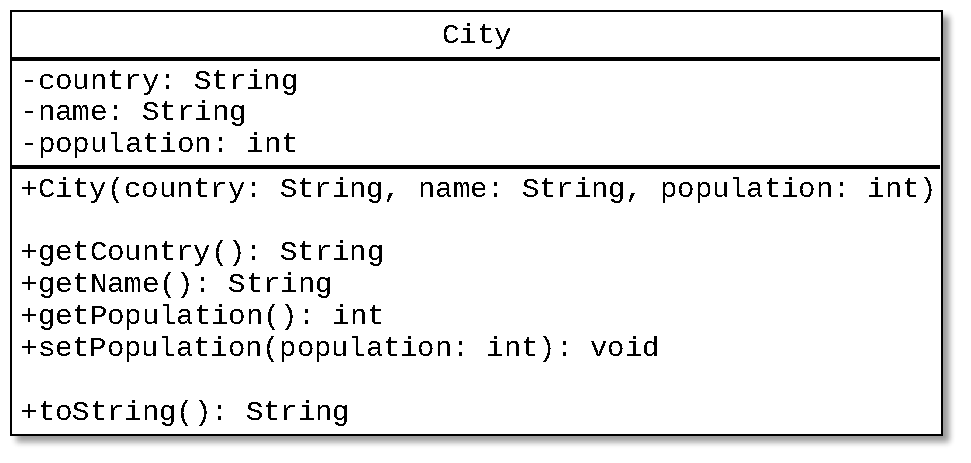
\includegraphics[scale=0.75]{figs/ch18/city.pdf}
\caption{UML diagram showing attributes and methods of the City class}
\label{fig.ch18.cityUML}
\end{center}
\end{figure}


{\large\bf{The \java{CityInfo} class}}

Then, write a class named \java{CityInfo} that contains the \java{main()} method.Use the {\em citylist.dat} file\footnotemark to set up the initial list of cities. The file is available from the repository at {\em ch18/citylist.dat} Each line of the text file has a country code, city name, and population, separated by semicolons. Your program must first read the city data file with this method:

\footnotetext{The data for this exercise came from \url{http://geonames.org/}, licensed under a Creative Commons Attribution 4.0 License (see \url{https://creativecommons.org/licenses/by/4.0/})}

\begin{stdout}
public static ArrayList<City> readCityFile(String fileName)
\end{stdout}

This method will open the given \java{fileName}, read it, and return an \java{ArrayList} of \java{City} objects corresponding to each line of the file.

If a line in the file has bad data (non-numeric population or too many or too few entries), your program will print an error that displays the bad line without entering any new data into the \java{ArrayList}. The \java{citylist.dat} file in the repository purposely contains some lines with bad data so you can test to see if your error-handling code works. Do not write your code for this specific file; another person's file might have bad data on different lines with different data on them.

If the file does not exist, the method prints an appropriate error message and returns an empty \java{ArrayList<City>}.

If the returned \java{ArrayList} is not empty, the program will repeatedly ask for a country code (or ENTER to quit).
Once the user enters a country code, the \java{main()} method will call this method:

\begin{stdout}
public static int statistics(String countryCode,
   ArrayList<City> cityList)
\end{stdout}

The \java{statistics()} method will go through the city list and

\begin{itemize}
    \item Calculate the total number of cities in the given country.
    \item If there are more than zero cities:
        \begin{itemize}
            \item Print the total number of cities
            \item Print the average population for those cities
        \end{itemize}
    
    \item Otherwise, prints an appropriate error message.
    \item Returns the total number of cities found.
\end{itemize}

The \java{main()} method will then use this returned value. If it is greater than zero, you will write a new file name {\em CC.dat}, where {\em CC} stands for a country code. This file will have the information for the cities in that country in the same format as \java{citylist.dat}. For example, if the country code is \java{JP}, your program will create a file named {\em JP.dat}. You will use a method named

\begin{stdout}
public static void writeCountryFile(String countryCode,
    ArrayList<City> cityList)
\end{stdout}

to do this. If there is an \java{IOException} while opening the output file or writing the data, print an appropriate error message. You must use the exception's \java{getMessage()} method when constructing your error message. If the file is written successfully, print a message letting the user know that the file has been created. This message {\em must} contain the file name.

{\large\bf{Handling Exceptions}}

Your program must handle these exceptions:

\begin{itemize}
    \item Catch \java{FileNotFoundException}when opening a \java{Scanner} for the input file. You could use the \java{File.exists()} method, but let's use exceptions to get more practice.)
    \item Catch \java{NumberFormatException} when reading the input file and converting strings to numbers.
    \item You will probably need nested \java{try}/\java{catch} blocks for file input: one outside the read loop when opening the file, and one inside the read loop to skip badly formatted lines.
    \item Catch \java{IOException} when writing an output file.
\end{itemize}

Here are some things to note:

\begin{itemize}
    \item You must accept input in either upper or lower case.
    \item You will need to loop through the \java{cityList} twice; once in \java{statistics()} to get the total and average (if applicable), and again in \java{writeCountryFile()} to create the output file. This is a design decision---I decided these are two separate tasks to be done by two methods, rather than combining both tasks into one method.
\end{itemize}

Here is what the program output might look like. Your output does not have to look exactly like this, but it must reflect the same information.

\begin{stdout}
Reading city file...
"AB;Too few" does not have three entries.
"CD;Too many;1056382;extra" does not have three entries.
"EF;Bad number;one million" does not have a number on it.

Enter a two-letter country code, or press ENTER to quit: UA
Number of cities in UA: 5
Average population is 1,457,504.
File UA.dat written successfully.
Enter a two-letter country code, or press ENTER to quit: LU
No cities found in LU.
Enter a two-letter country code, or press ENTER to quit: MX
Number of cities in MX: 11
Average population is 2,427,622.
File MX.dat written successfully.
Enter a two-letter country code, or press ENTER to quit: 
\end{stdout}

Here are the contents of the file {\em UA.dat}

\begin{stdout}
UA;Kiev;2797553
UA;Kharkiv;1430885
UA;Dnipropetrovsk;1032822
UA;Donets'k;1024700
UA;Odessa;1001558
\end{stdout}

Here is an example of the output you might get for an error while writing the file (I deliberately caused this error by changing my directory to be read-only).

\begin{stdout}
Error writing FR.dat
FR.dat (Permission denied)
\end{stdout}

\end{exercise}

\begin{exercise}
In this exercise, you will write two classes: a class that represents a bank account and a program that works like an ATM for bank accounts. The code repository has some pseudocode in file {\em ch18/ATM\_Pseudocode.java} that may help you get the program organized and started. 

{\large\bf{The \java{Account} class}}

First, create an \java{Account} class. An \java{Account} object has these properties:

\begin{itemize}
    \item \java{private int acctNumber}: the account number
    \item \java{private String name}: the account holder's name
    \item \java{private double balance}: the current balance in the account
\end{itemize}

Implement these methods:

\begin{description}
    \item[\texttt{public Account(int acctNumber, String name, double balance)}] \hfill \\ The constructor
    \item[\texttt{public String toString()}] \hfill \\  Returns a string giving the account ID, name, and balance, separated by colons. Do not use \java{format()} on the balance; you want to keep the number as accurate as possible.
    \item[\texttt{public void deposit(double amount)}] \hfill \\  Adds the given amount to the current balance. If the amount is negative, the balance must not be changed; otherwise, the \java{balance} property is updated to reflect the deposit.
    \item[\texttt{public void withdraw(double amount)}] \hfill \\ Withdraws the given amount from the current balance. If the amount is negative or greater than the current balance, the balance must not be changed; otherwise, the \java{balance} is updated to reflect the withdrawal.
\end{description}

You must also write a getter and setter for the balance, and only a getter for the name and account number; once the account is constructed, the name and account number never change. The getters and setters must be \java{public}.

Note that \java{deposit()} and \java{withdraw()} do not print error messages if they get incorrect input; they simply ignore it. It is up to the program that calls these functions to provide the error messages for the user of the program.

{\large\bf{The \java{Customer} class}}

Next, write a program named \java{Customer.java} that has a \java{main()} method. This class provides an ``ATM''-like interface to a set of bank accounts. Use the following {\em accounts.dat} file to set up the initial set of accounts. Each line of the text file has an account ID, name, and starting balance, separated by colons. Your program must first read the account data file and build an \java{ArrayList} of \java{Account} objects corresponding to each line. If the file does not exist, your program must output a reasonable error message and then quit.

\begin{stdout}
15725:Christina Plaka:456.71
23981:Roz Chast:1853.22
57012:Georges Remi:3571.85
46287:Raquel Corcoles:783.00
31954:Eiichiro Oda:854.02
84373:Scott McCloud:2733.96
\end{stdout}

If the file is read successfully, the program will repeatedly ask for an account number (or ENTER to quit). This is equivalent to inserting an ATM card. Repeat until the account number is valid. Hint: write a method like this:

\begin{stdout}
public static int findIndex(ArrayList<Account> accountList,
   int accountNumber)
\end{stdout}

This method will go through the \java{accountList} and return the index of the account with the given \java{accountNumber}, or -1 if the account number does not belong to any of the accounts in the array.

Print a message that greets the customer by name. Then repeatedly ask the customer if they want to deposit, withdraw, or finish the transactions.

\begin{itemize}
    \item If the customer wishes to deposit, ask for the amount until you get a number greater than or equal to zero; then perform the transaction and display the balance. Print an appropriate message for invalid input. You must handle exceptions here.
    \item If the customer wishes to withdraw, ask for the amount until you get a number greater than or equal to zero and less than or equal to the current balance; then perform the transaction and display the balance. Print an appropriate message for invalid input. You must handle exceptions here.
    \item If the customer is finished, print a message to say goodbye to the customer, write the entire account array back to disk, and return to the account number prompt. (This is equivalent to giving the customer their card back).
\end{itemize}

This program must print all monetary amounts preceded by a dollar sign and with two digits after the decimal point. This is where you {\em do} want to use \java{format} to round to two decimal places.

{\large\bf{Handling Exceptions}}

Your program must handle exceptions when opening the {\em accounts.dat} file. It must produce a reasonable error message and quit rather than crashing if the file doesn't exist.

Your program must also handle exceptions if the user enters invalid input such as``fifteen'' for the account number or amount to deposit/withdraw.

The exceptions you will probably want to use the most are \java{java.IO.IOException} for file errors and \java{NumberFormatException} for invalid numbers.

Here is what you might see as output when you run your program:

\begin{stdout}
Enter your account number: 12345
Unknown account number
Enter your account number: five
five is not a number
Enter your account number: 57012
Hello, Georges Remi!
Your current balance is $3571.85
D)eposit, W)ithdraw, or F)inish? D
Enter amount to deposit: $-20
You cannot deposit a negative amount.
D)eposit, W)ithdraw, or F)inish? D
Enter amount to deposit: $fifty
fifty is not a valid number.
D)eposit, W)ithdraw, or F)inish? D
Enter amount to deposit: $50
Your current balance is $3621.85
D)eposit, W)ithdraw, or F)inish? w
Enter amount to withdraw: $-200
You cannot withdraw a negative amount.
D)eposit, W)ithdraw, or F)inish? w
Enter amount to withdraw: $570.00
Your current balance is $3051.85
D)eposit, W)ithdraw, or F)inish? f
Goodbye, Georges Remi.

Enter your account number: 23981
Hello, Roz Chast!
Your current balance is $1853.22
D)eposit, W)ithdraw, or F)inish? w
Enter amount to withdraw: $1890
You cannot withdraw more than you have.
D)eposit, W)ithdraw, or F)inish? w
Enter amount to withdraw: $80
Your current balance is $1773.22
D)eposit, W)ithdraw, or F)inish? f
Goodbye, Roz Chast.

Enter your account number:
ATM program concludes.
\end{stdout}

After you finish running this program, the {\em accounts.dat} file will have the new balance(s):

\begin{stdout}
15725:Christina Plaka:456.71
23981:Roz Chast:1773.22
57012:Georges Remi:3051.85
46287:Raquel Corcoles:783.0
31954:Eiichiro Oda:854.02
84373:Scott McCloud:2733.96
\end{stdout}

\end{exercise}


\appendix
%\addtocontents{toc}{\protect\newpage}

%~ \part{Appendixes}

%BEGIN LATEX
\renewcommand{\chaptermark}[1]{\markboth{Appendix \thechapter ~~ #1}{}}
%END LATEX

\chapter{Path Names}
\label{pathnames}

\section{Absolute Paths}

Imagine your file hierarchy as a map, where folders represents streets and files represent houses, as in Figure~\ref{fig.files}.

\begin{figure}[!ht]
\begin{center}
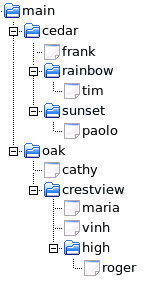
\includegraphics[width=0.2\textwidth]{figs/streets.png}
\caption{A Tree of Directories and Files}
\label{fig.files}
\end{center}
\end{figure}

An absolute pathname is like giving directions starting at the very outside of the map and working inwards. The directions for getting to Maria's house in an absolute fashion would be ``Start at Main street, then go to Oak street, then to Crestview Drive, and there is Maria's house.'' In terms of Linux or Mac OS pathnames, that would be \texttt{/main/oak/crestview/maria}.

In Linux and Mac OS, the / (slash) separates levels of directory. The topmost level of the file system has no name, so when you start from the topmost level, you start with a separator---the slash.

The absolute pathname to get to Frank's house is ``Start at Main Street, go to Cedar Street, and there is Frank's house.'' (\texttt{/main/cedar/frank}).

On Windows, if all these files were on the \texttt{C:} drive, the absolute path would be \texttt{C:\textbackslash main\textbackslash cedar\textbackslash frank}.

\section{Relative Paths}

Now let's say you were on Crestview Drive in front of Maria's house and someone asked you how to get to Vinh's house. You wouldn't answer, ``Start at Main Street, then go to Oak Street, then go to Crestview Drive...'' You wouldn't do that because you're already on the correct street. You would just say ``Vinh's house is next door.'' That is a {\em relative pathname}---starting from where you are right now, how do you get to the destination? When specifying a Java path, if you are in directory \texttt{/main/oak/crestview}, the relative filename for file \texttt{vinh} is just that: \texttt{vinh}, because it is in your current directory.

If you were on Cedar Street and someone asked you how to get to Tim's house, you would tell them to go to Rainbow Drive, and there's Tim's house. The relative path is \texttt{rainbow/tim}. On Linux or Mac OS, relative pathnames {\em never} begin with a slash; on Windows they {\em never} begin with a drive name.

If you were on Oak Street and someone asked you how to get to High Street, you would answer with a relative path: Go to Crestview Drive, and from there to High Street. As a relative path, that's \texttt{crestview/high}.

Now comes a tricky one. You're on Sunset Drive (in the diagram, that is the vertical dotted line beneath the folder labeled \texttt{sunset}), and someone asks you how to get to Frank's house. You have to say: ``Go back up one street (that puts you on Cedar street, the vertical dotted line under the \texttt{cedar} folder); that's where you will find Frank's house.'' Whenever you tell someone to go back up one level in the file hierarchy, you use two dots \texttt{..} to symbolize the parent directory. In Linux terms, the relative pathname is \texttt{../frank}

Important: The relative pathname is not \texttt{cedar/frank}. If you are on Sunset Drive, you can't go directly to Cedar Street; it's not one of your sub-directories.

Using \texttt{../cedar/frank} is also incorrect. That would mean ``back up one level (which puts you on Cedar street) and then go to Cedar street (but you can't; inside the \texttt{cedar} folder there is no other folder named \texttt{cedar}!)

You can use \texttt{..} as often as you need to in a relative path. If you are on Rainbow Drive and want to go to Cathy's house, you have to back up to Cedar Street, and from there back up to Main Street. Once there, you have a straight shot to Oak Street and Cathy's house. Thus, the relative path is \texttt{../../oak/cathy}

There is one other abbreviation you can use in Java paths: the dot \texttt{.} means ``my current directory,'' so if you were to use the path \texttt{./example.txt}, it would be a relative path name to the file \texttt{example.txt} in the current directory, exactly the same as \texttt{example.txt}. This seems redundant, but the ``my current directory'' concept is often convenient when using the command line interface in Mac OS or Linux. 


\backmatter

\printindex

%-------------------------------------------------------------
\ifplastex
\else

\newpage
\thispagestyle{empty}

\vspace*{40pt}

{\bf\huge About the Author}

{\bf J. David Eisenberg} teaches Computer Science at Evergreen Valley College in San Jos\'e, California. He has authored and co-authored several books: {\it SVG Essentials}, {\it \'Etudes for Erlang}, and {\it Web Development with ReasonML}.

\vspace*{40pt}

{\bf\huge About the Authors of {\em Think Java}}

{\bf Allen Downey} is a professor of computer science at Olin College of Engineering.
He has taught computer science at Wellesley College, Colby College, and UC Berkeley.
He has a PhD in computer science from UC Berkeley and master's and bachelor's degrees from MIT.
Allen is the creator of the best-selling Think series for O'Reilly, which includes {\it Think Python}, {\it Think Complexity}, {\it Think DSP}, and {\it Think Bayes}.

{\bf Chris Mayfield} is an associate professor of computer science at James Madison University, with a research focus on CS education and professional development.
He has a PhD in computer science from Purdue University and bachelor's degrees in CS and German from the University of Utah.

\fi
\end{document}
